%%%%%%%%%
% Change year here
\def\currentcohort{2016 / 2017}
%%%%%%%%%%%%


%nothing from here on should be changed!!!


\documentclass[a4paper,fleqn,12pt]{book} %general structure
%----------------------------------------------------------------------------------------
%	VARIOUS REQUIRED PACKAGES
%----------------------------------------------------------------------------------------

\usepackage{titlesec} % Allows customization of titles

\usepackage{enumitem} % Customize lists
\setlist{nolistsep} % Reduce spacing between bullet points and numbered lists

%----------------------------------------------------------------------------------------
%	MAIN TABLE OF CONTENTS
%----------------------------------------------------------------------------------------

\usepackage{titletoc} % Required for manipulating the table of contents

\contentsmargin{0cm} % Removes the default margin
% Chapter text styling
\titlecontents{chapter}[1.25cm] % Indentation
{\addvspace{15pt}\large\sffamily\bfseries} % Spacing and font options for chapters
{\color{titlepagecolour!60}\contentslabel[\Large\thecontentslabel]{1.25cm}\color{titlepagecolour}} % Chapter number
{}  
{\color{titlepagecolour!60}\normalsize\sffamily\bfseries\;\titlerule*[.5pc]{.}\;\thecontentspage} % Page number
% Section text styling
\titlecontents{section}[1.25cm] % Indentation
{\addvspace{5pt}\sffamily\bfseries} % Spacing and font options for sections
{\contentslabel[\thecontentslabel]{1.25cm}} % Section number
{}
{\sffamily\hfill\color{black}\thecontentspage} % Page number
[]
% Subsection text styling
\titlecontents{subsection}[1.25cm] % Indentation
{\addvspace{1pt}\sffamily\small} % Spacing and font options for subsections
{\contentslabel[\thecontentslabel]{1.25cm}} % Subsection number
{}
{\sffamily\;\titlerule*[.5pc]{.}\;\thecontentspage} % Page number
[] 

%----------------------------------------------------------------------------------------
%	MINI TABLE OF CONTENTS IN CHAPTER HEADS
%----------------------------------------------------------------------------------------

% Section text styling
\titlecontents{lsection}[0em] % Indendating
{\footnotesize\sffamily} % Font settings
{}
{}
{}

% Subsection text styling
\titlecontents{lsubsection}[.5em] % Indentation
{\normalfont\footnotesize\sffamily} % Font settings
{}
{}
{}
 
%----------------------------------------------------------------------------------------
%	PAGE HEADERS
%----------------------------------------------------------------------------------------

\usepackage{fancyhdr} % Required for header and footer configuration

\pagestyle{fancy}
\renewcommand{\chaptermark}[1]{\markboth{\sffamily\normalsize\bfseries\chaptername\ \thechapter.\ #1}{}} % Chapter text font settings
\renewcommand{\sectionmark}[1]{\markright{\sffamily\normalsize\thesection\hspace{5pt}#1}{}} % Section text font settings
\fancyhf{} \fancyhead[LE,RO]{\sffamily\normalsize\thepage} % Font setting for the page number in the header
\fancyhead[LO]{\rightmark} % Print the nearest section name on the left side of odd pages
\fancyhead[RE]{\leftmark} % Print the current chapter name on the right side of even pages
\renewcommand{\headrulewidth}{0.5pt} % Width of the rule under the header
\addtolength{\headheight}{2.5pt} % Increase the spacing around the header slightly
\renewcommand{\footrulewidth}{0pt} % Removes the rule in the footer
\fancypagestyle{plain}{\fancyhead{}\renewcommand{\headrulewidth}{0pt}} % Style for when a plain pagestyle is specified

% Removes the header from odd empty pages at the end of chapters
\makeatletter
\renewcommand{\cleardoublepage}{
\clearpage\ifodd\c@page\else
\hbox{}
\vspace*{\fill}
\thispagestyle{empty}
\newpage
\fi}

%----------------------------------------------------------------------------------------
%	THEOREM STYLES
%----------------------------------------------------------------------------------------

\usepackage{amsmath,amsfonts,amssymb,amsthm} % For math equations, theorems, symbols, etc

\newcommand{\intoo}[2]{\mathopen{]}#1\,;#2\mathclose{[}}
\newcommand{\ud}{\mathop{\mathrm{{}d}}\mathopen{}}
\newcommand{\intff}[2]{\mathopen{[}#1\,;#2\mathclose{]}}
\newtheorem{notation}{Notation}[chapter]

%%%%%%%%%%%%%%%%%%%%%%%%%%%%%%%%%%%%%%%%%%%%%%%%%%%%%%%%%%%%%%%%%%%%%%%%%%%
%%%%%%%%%%%%%%%%%%%% dedicated to boxed/framed environements %%%%%%%%%%%%%%
%%%%%%%%%%%%%%%%%%%%%%%%%%%%%%%%%%%%%%%%%%%%%%%%%%%%%%%%%%%%%%%%%%%%%%%%%%%
\newtheoremstyle{titlepagecolournumbox}% % Theorem style name
{0pt}% Space above
{0pt}% Space below
{\normalfont}% % Body font
{}% Indent amount
{\small\bf\sffamily\color{titlepagecolour}}% % Theorem head font
{\;}% Punctuation after theorem head
{0.25em}% Space after theorem head
{\small\sffamily\color{titlepagecolour}\thmname{#1}\nobreakspace\thmnumber{\@ifnotempty{#1}{}\@upn{#2}}% Theorem text (e.g. Theorem 2.1)
\thmnote{\nobreakspace\the\thm@notefont\sffamily\bfseries\color{black}---\nobreakspace#3.}} % Optional theorem note
\renewcommand{\qedsymbol}{$\blacksquare$}% Optional qed square

\newtheoremstyle{blacknumex}% Theorem style name
{5pt}% Space above
{5pt}% Space below
{\normalfont}% Body font
{} % Indent amount
{\small\bf\sffamily}% Theorem head font
{\;}% Punctuation after theorem head
{0.25em}% Space after theorem head
{\small\sffamily{\tiny\ensuremath{\blacksquare}}\nobreakspace\thmname{#1}\nobreakspace\thmnumber{\@ifnotempty{#1}{}\@upn{#2}}% Theorem text (e.g. Theorem 2.1)
\thmnote{\nobreakspace\the\thm@notefont\sffamily\bfseries---\nobreakspace#3.}}% Optional theorem note

\newtheoremstyle{blacknumbox} % Theorem style name
{0pt}% Space above
{0pt}% Space below
{\normalfont}% Body font
{}% Indent amount
{\small\bf\sffamily}% Theorem head font
{\;}% Punctuation after theorem head
{0.25em}% Space after theorem head
{\small\sffamily\thmname{#1}\nobreakspace\thmnumber{\@ifnotempty{#1}{}\@upn{#2}}% Theorem text (e.g. Theorem 2.1)
\thmnote{\nobreakspace\the\thm@notefont\sffamily\bfseries---\nobreakspace#3.}}% Optional theorem note

%%%%%%%%%%%%%%%%%%%%%%%%%%%%%%%%%%%%%%%%%%%%%%%%%%%%%%%%%%%%%%%%%%%%%%%%%%%
%%%%%%%%%%%%% dedicated to non-boxed/non-framed environements %%%%%%%%%%%%%
%%%%%%%%%%%%%%%%%%%%%%%%%%%%%%%%%%%%%%%%%%%%%%%%%%%%%%%%%%%%%%%%%%%%%%%%%%%
\newtheoremstyle{titlepagecolournum}% % Theorem style name
{5pt}% Space above
{5pt}% Space below
{\normalfont}% % Body font
{}% Indent amount
{\small\bf\sffamily\color{titlepagecolour}}% % Theorem head font
{\;}% Punctuation after theorem head
{0.25em}% Space after theorem head
{\small\sffamily\color{titlepagecolour}\thmname{#1}\nobreakspace\thmnumber{\@ifnotempty{#1}{}\@upn{#2}}% Theorem text (e.g. Theorem 2.1)
\thmnote{\nobreakspace\the\thm@notefont\sffamily\bfseries\color{black}---\nobreakspace#3.}} % Optional theorem note
\renewcommand{\qedsymbol}{$\blacksquare$}% Optional qed square
\makeatother

% Defines the theorem text style for each type of theorem to one of the three styles above
\newcounter{dummy} 
\numberwithin{dummy}{section}
\theoremstyle{titlepagecolournumbox}
\newtheorem{theoremeT}[dummy]{Theorem}
\newtheorem{problem}{Problem}[chapter]
\newtheorem{exerciseT}{Exercise}[chapter]
\theoremstyle{blacknumex}
\newtheorem{exampleT}{Example}[chapter]
\theoremstyle{blacknumbox}
\newtheorem{vocabulary}{Vocabulary}[chapter]
\newtheorem{definitionT}{Definition}[section]
\newtheorem{corollaryT}[dummy]{Corollary}
\theoremstyle{titlepagecolournum}
\newtheorem{proposition}[dummy]{Proposition}

%----------------------------------------------------------------------------------------
%	DEFINITION OF COLORED BOXES
%----------------------------------------------------------------------------------------

\RequirePackage[framemethod=default]{mdframed} % Required for creating the theorem, definition, exercise and corollary boxes

% Theorem box
\newmdenv[skipabove=7pt,
skipbelow=7pt,
backgroundcolor=black!5,
linecolor=titlepagecolour,
innerleftmargin=5pt,
innerrightmargin=5pt,
innertopmargin=5pt,
leftmargin=0cm,
rightmargin=0cm,
innerbottommargin=5pt]{tBox}

% Exercise box	  
\newmdenv[skipabove=7pt,
skipbelow=7pt,
rightline=false,
leftline=true,
topline=false,
bottomline=false,
backgroundcolor=titlepagecolour!10,
linecolor=titlepagecolour,
innerleftmargin=5pt,
innerrightmargin=5pt,
innertopmargin=5pt,
innerbottommargin=5pt,
leftmargin=0cm,
rightmargin=0cm,
linewidth=4pt]{eBox}	

% Definition box
\newmdenv[skipabove=7pt,
skipbelow=7pt,
rightline=false,
leftline=true,
topline=false,
bottomline=false,
linecolor=titlepagecolour,
innerleftmargin=5pt,
innerrightmargin=5pt,
innertopmargin=0pt,
leftmargin=0cm,
rightmargin=0cm,
linewidth=4pt,
innerbottommargin=0pt]{dBox}	

% Corollary box
\newmdenv[skipabove=7pt,
skipbelow=7pt,
rightline=false,
leftline=true,
topline=false,
bottomline=false,
linecolor=gray,
backgroundcolor=black!5,
innerleftmargin=5pt,
innerrightmargin=5pt,
innertopmargin=5pt,
leftmargin=0cm,
rightmargin=0cm,
linewidth=4pt,
innerbottommargin=5pt]{cBox}

% Creates an environment for each type of theorem and assigns it a theorem text style from the "Theorem Styles" section above and a colored box from above
\newenvironment{theorem}{\begin{tBox}\begin{theoremeT}}{\end{theoremeT}\end{tBox}}
\newenvironment{exercise}{\begin{eBox}\begin{exerciseT}}{\hfill{\color{titlepagecolour}\tiny\ensuremath{\blacksquare}}\end{exerciseT}\end{eBox}}				  
\newenvironment{definition}{\begin{dBox}\begin{definitionT}}{\end{definitionT}\end{dBox}}	
\newenvironment{example}{\begin{exampleT}}{\hfill{\tiny\ensuremath{\blacksquare}}\end{exampleT}}		
\newenvironment{corollary}{\begin{cBox}\begin{corollaryT}}{\end{corollaryT}\end{cBox}}	

%----------------------------------------------------------------------------------------
%	REMARK ENVIRONMENT
%----------------------------------------------------------------------------------------

\newenvironment{remark}{\par\vspace{10pt}\small % Vertical white space above the remark and smaller font size
\begin{list}{}{
\leftmargin=35pt % Indentation on the left
\rightmargin=25pt}\item\ignorespaces % Indentation on the right
\makebox[-2.5pt]{\begin{tikzpicture}[overlay]
\node[draw=titlepagecolour!60,line width=1pt,circle,fill=titlepagecolour!25,font=\sffamily\bfseries,inner sep=2pt,outer sep=0pt] at (-15pt,0pt){\textcolor{titlepagecolour}{R}};\end{tikzpicture}} % Orange R in a circle
\advance\baselineskip -1pt}{\end{list}\vskip5pt} % Tighter line spacing and white space after remark

%----------------------------------------------------------------------------------------
%	SECTION NUMBERING IN THE MARGIN
%----------------------------------------------------------------------------------------

\makeatletter
\renewcommand{\@seccntformat}[1]{\llap{\textcolor{titlepagecolour}{\csname the#1\endcsname}\hspace{1em}}}                    
\renewcommand{\section}{\@startsection{section}{1}{\z@}
{-4ex \@plus -1ex \@minus -.4ex}
{1ex \@plus.2ex }
{\normalfont\large\sffamily\bfseries}}
\renewcommand{\subsection}{\@startsection {subsection}{2}{\z@}
{-3ex \@plus -0.1ex \@minus -.4ex}
{0.5ex \@plus.2ex }
{\normalfont\sffamily\bfseries}}
\renewcommand{\subsubsection}{\@startsection {subsubsection}{3}{\z@}
{-2ex \@plus -0.1ex \@minus -.2ex}
{.2ex \@plus.2ex }
{\normalfont\small\sffamily\bfseries}}                        
\renewcommand{\paragraph}{\@startsection{paragraph}{4}{\z@}
{-2ex \@plus-.2ex \@minus .2ex}
{.1ex}
{\normalfont\small\sffamily\bfseries}}

%----------------------------------------------------------------------------------------
%	HYPERLINKS IN THE DOCUMENTS
%----------------------------------------------------------------------------------------

% For an unclear reason, the package should be loaded now and not later
\usepackage[pdftex,
            pdfauthor={New College MCR},
            pdftitle={MCR Freshers' Guide \currentcohort},
            pdfproducer={TeXLive 2014 via TeXlipse},
            pdfcreator={pdflatex},
            hidelinks,
            colorlinks=true,
            breaklinks=false,
            linkcolor=,
            urlcolor= titlepagecolour,
            linktocpage=true]{hyperref}

%----------------------------------------------------------------------------------------
%	CHAPTER HEADINGS
%----------------------------------------------------------------------------------------

% The set-up below should be (sadly) manually adapted to the overall margin page septup controlled by the geometry package loaded in the main.tex document. It is possible to implement below the dimensions used in the goemetry package (top,bottom,left,right)... TO BE DONE

\newcommand{\thechapterimage}{}
\newcommand{\chapterimage}[1]{\renewcommand{\thechapterimage}{#1}}

% Numbered chapters with mini tableofcontents
\def\thechapter{\arabic{chapter}}
\def\@makechapterhead#1{
\thispagestyle{empty}
{\centering \normalfont\sffamily
\ifnum \c@secnumdepth >\m@ne
\if@mainmatter
\startcontents
\begin{tikzpicture}[remember picture,overlay]
\node at (current page.north west)
{\begin{tikzpicture}[remember picture,overlay]
\node[anchor=north west,inner sep=0pt] at (0,0) {\includegraphics[width=\paperwidth]{\thechapterimage}};
%%%%%%%%%%%%%%%%%%%%%%%%%%%%%%%%%%%%%%%%%%%%%%%%%%%%%%%%%%%%%%%%%%%%%%%%%%%%%%%%%%%%%
% Commenting the 3 lines below removes the small contents box in the chapter heading
\ifnum \c@nosmtoc =\@ne
\else
\fill[color=titlepagecolour!10!white,opacity=.6] (1cm,0) rectangle (8cm,-4.8cm);
\node[anchor=north west] at (1.1cm,.35cm)
{\parbox[t][8cm][t]{4.5cm}{\huge\bfseries\flushleft \printcontents{l}{1}{\setcounter{tocdepth}{1}}}}; 
\fi
\draw[anchor=west] (5cm,-9cm) node [rounded corners=20pt,fill=titlepagecolour!10!white,text opacity=1,draw=titlepagecolour,draw opacity=1,line width=1.5pt,fill opacity=.6,inner sep=15pt]{\huge\sffamily\bfseries\textcolor{black}{\thechapter. #1\strut\makebox[22cm]{}}};
%%%%%%%%%%%%%%%%%%%%%%%%%%%%%%%%%%%%%%%%%%%%%%%%%%%%%%%%%%%%%%%%%%%%%%%%%%%%%%%%%%%%%
\end{tikzpicture}};
\end{tikzpicture}}
\par\vspace*{230\p@}
\fi
\fi}



\makeatother % Insert the commands.tex file which contains the majority of
% the structure behind the main body template
\usepackage{tikz} %used to draw shapes on title page and chapter headings
\usepackage{libertine} %use non-standard font (especially for cover)
\usepackage[T1]{fontenc} %font formatting
\usepackage{eso-pic} %cover background
\usepackage{xcolor} %colours
\usepackage{microtype} % Slightly tweak font spacing for aesthetics
\usepackage[utf8]{inputenc} % Required for including letters with accents
\usepackage{calc} % For simpler calculation - used for spacing the index letter headings correctly
\usepackage[top=3cm,bottom=3cm,left=3.2cm,right=3.2cm,headsep=10pt,a4paper]{geometry}% modified margins
\usepackage[english]{babel} %spelling, hyphenation
\usepackage{graphicx} %needed for pictures
\usepackage{booktabs} %nicer tables
\usepackage{array} %formatting of tables
\usepackage[notlof]{tocbibind} %lists all those tables of contents in the table
%of content, which do not reference themselves ;)
\usepackage{pdfpages} %college map
\usepackage{caption} %captionof command
\usepackage{wrapfig} %text and picture ide by side
\usepackage{tabularx}
\usepackage{grffile}

\addto\captionsenglish{\renewcommand{\figurename}{Fig.}} %change label for figures
\addto\captionsenglish{\renewcommand{\listfigurename}{\biolinum \Large
\textcolor{titlepagecolour}{Credit must go where credit is due}}}% modify lof name

\graphicspath{{Pictures/}} %put all pictures into folder ``Pictures''

\usetikzlibrary[positioning] %positioning of purple blocks, chapter heading boxes etc

\renewcommand\UrlFont{\rmfamily\itshape} %font used for URLs/clickable links

\definecolor{titlepagecolour}{cmyk}{0.436,.865,0,.478} %primary colour used
\newcommand\urlformat[2]{{\color{titlepagecolour}#2\UrlFont#1}} %used for
% typesetting hidden URLs, i.e. \href{URL}{\urlformat{displayed}} results in a
% purple, italic word ``displayed'', which is a clickable link to ``URL''.
%%%%%%%%%%%%%%%%%%%%%%%%%%%%%%%%%%%%%%%%%%%%%%%%%%%%%%%%%%%%%%%%%%%%
%title page main layout
\newcommand\titlepagedecoration[1]{%
\begin{tikzpicture}[remember picture,overlay,shorten >= -10pt]
\coordinate (tp1) at ([yshift=3cm]current page.west);
\coordinate (tp2) at ([yshift=3cm,xshift=10cm]current page.west);
\coordinate (tp3) at ([yshift=0pt,xshift=12cm]current page.north);
\coordinate (tp4) at ([yshift=0pt]current page.north west);
\coordinate (tpx) at ([yshift=8cm,xshift=13cm]current page.west); 
\coordinate (tpy) at ([yshift=8cm,xshift=0cm]current page.west);
\coordinate (tpa) at (current page.south west);
\coordinate (tpb) at ([xshift=5cm]current page.south west);
\coordinate (tpc) at ([yshift=3cm,xshift=5cm]current page.west);
\coordinate (tpcenter) at ([xshift=2.5cm,yshift=8.8cm] current page.south west);

\filldraw[draw=titlepagecolour!60!white,fill=titlepagecolour!60!white] (tpa)--(tpb)--(tpc)--(tp1)--cycle;
\filldraw[draw=titlepagecolour,fill=titlepagecolour] (tp1)--(tp2)--(tp3)--(tp4)--cycle; 
\filldraw[draw=titlepagecolour!30!white,fill=titlepagecolour!30!white,opacity=0.2] ([xshift=-5cm]tp1)--([xshift=-5cm]tp2)--([xshift=-5cm]tp3)--([xshift=-5cm]tp4)--cycle;
\filldraw[opacity=0.4,draw=titlepagecolour,fill=titlepagecolour] (tpy) -- (tpx) -- (tp2) -- (tp1) -- cycle;
\node [rotate=90,white] at (tpcenter) {\resizebox{16.7cm}{!}{\biolinum NEW
COLLEGE}}; \node[right] at ([xshift=1cm,yshift=-5cm]current page.north west)
{\parbox{\textwidth}{\color{white}#1}}; \end{tikzpicture}%
}
%%%%%%%%%%%%%%%%%%%%%%%%%%%%%%%%%%%%%%%%%%%%%%%%%%%%%%%%%%%%%%%%%%
\author{% for PDF tags
    New College MCR
    }
\title{% for PDF tags
	MCR Fresher's Guide \currentcohort
	}
    
    
\begin{document}

\newcounter{nosmtoc} %needed for small tables of content in chapter headers
\setcounter{nosmtoc}{0} %which are on by default

\frontmatter
%----------------------------------------------------------------------------------------
%	Titlepage
%----------------------------------------------------------------------------------------

\begin{titlepage}
    \titlepagedecoration{%
        \resizebox{11cm}{!}{\biolinum MCR Freshers' Guide}\par
        \vspace*{1cm}
        \resizebox{8cm}{!}{\biolinum\currentcohort}  
    }
    \null\vfill

\AddToShipoutPicture*{\put(-100,-10)%
{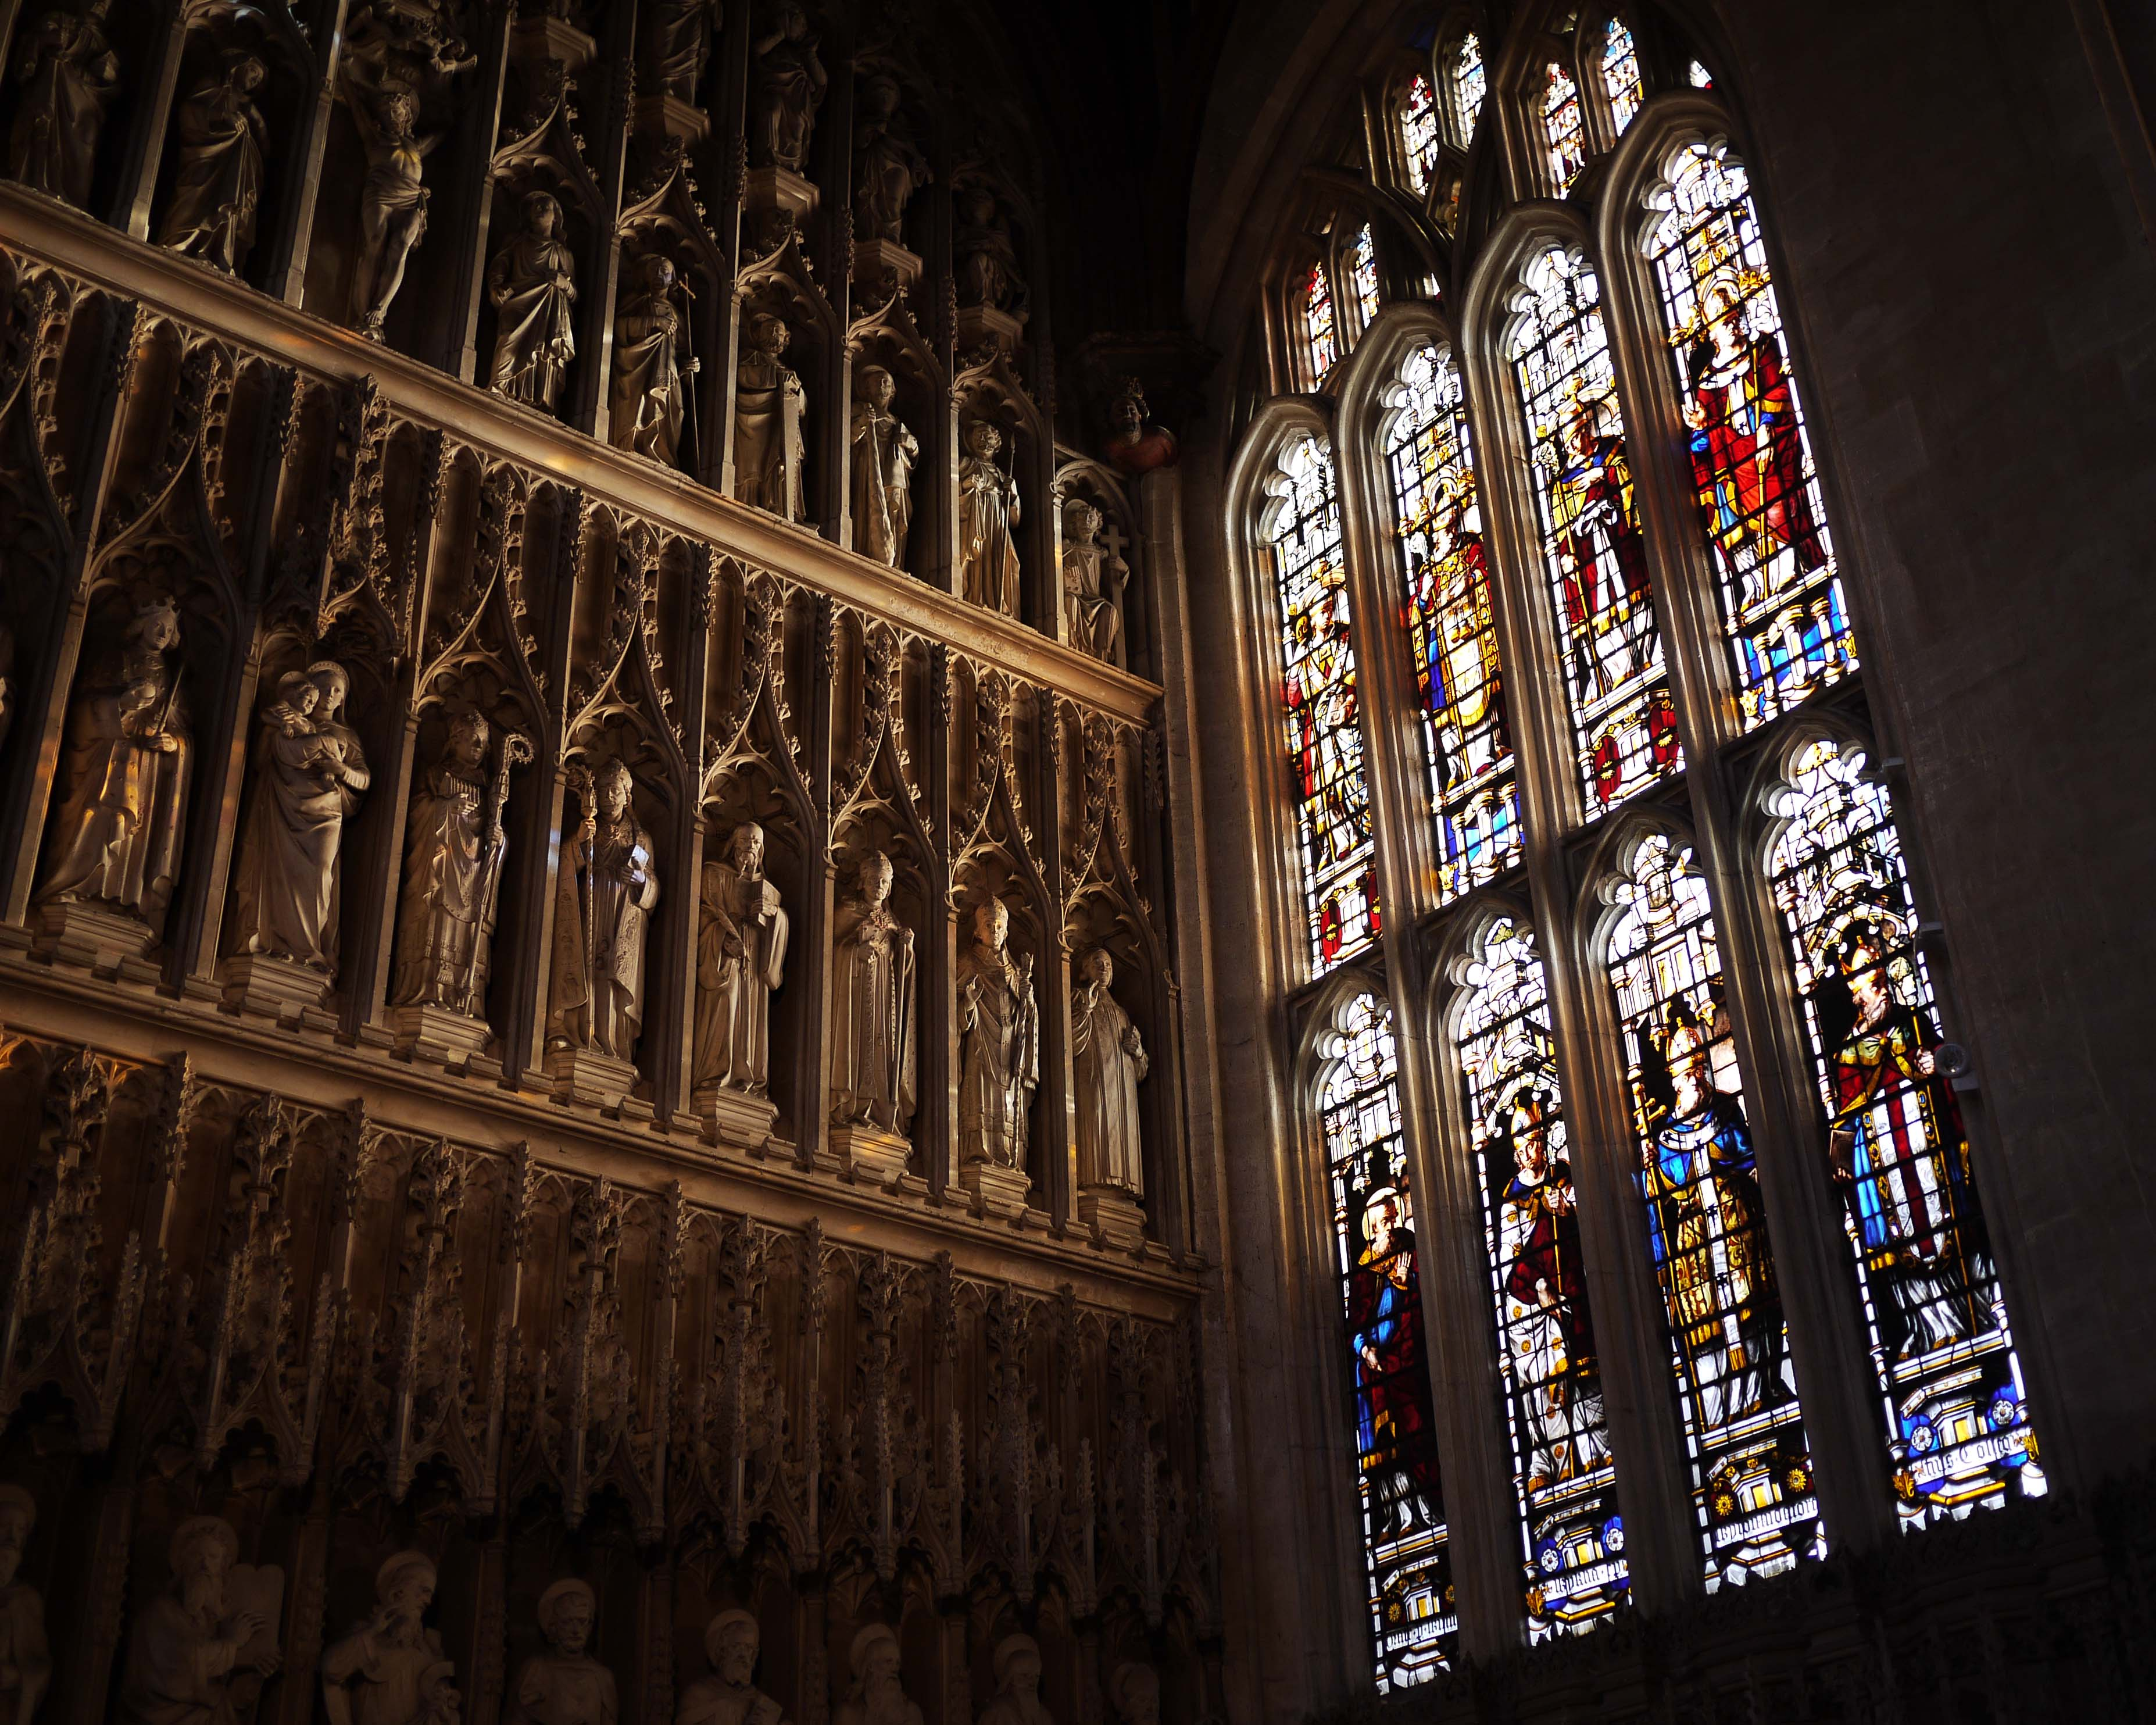
\includegraphics[scale=.28]{Title.jpg}% title page background
}} 
\AddToShipoutPicture*{\put(320,-255)%
{
\includegraphics[scale=0.3]{NCC.png}% faint College crest
}} 
\addcontentsline{lof}{figure}{Title page background: Photo credit to Naysan
Rafati/\href{http://oxonogaphy.wordpress.com}{Oxonography}}
\end{titlepage}

%----------------------------------------------------------------------------------------
%	COPYRIGHT PAGE
%----------------------------------------------------------------------------------------

\newpage
~\vfill

\thispagestyle{empty}
\enlargethispage{\baselineskip}

\listoffigures

\smallskip

\noindent Copyright \copyright\ 2014 New College MCR % Copyright notice
\smallskip

\noindent \url{http://mcr.new.ox.ac.uk/}\\ % URL

\noindent This guide builds on and modifies the
\href{http://www.latextemplates.com/template/the-legrand-orange-book}{\urlformat{The
Legrand Orange Book}} template originally written by \href{mailto:legrand.mathias@gmail.com}{\urlformat{Mathias
Legrand}}, subsequently edited by
\href{mailto:vel@latextemplates.com}{\urlformat{Vel}} for
\href{http://www.latextemplates.com/}{\urlformat{LaTeXTemplates.com}}, published
under a CC-NC-SA 3.0 licence. \\ %Attribution and Modification notice

\noindent Licensed under the Creative Commons Attribution-NonCommercial 3.0
Unported License (the ``License''). You may not use this file except in compliance with the License. You may obtain a copy of the License at \url{http://creativecommons.org/licenses/by-nc/3.0}. Unless required by applicable law or agreed to in writing, software distributed under the License is distributed on an \textsc{``as is'' basis, without warranties or conditions of any kind}, either express or implied. See the License for the specific language governing permissions and limitations under the License.\\ % License information

\noindent \textit{August 2014} % Printing/edition date

%----------------------------------------------------------------------------------------
%	TABLE OF CONTENTS
%----------------------------------------------------------------------------------------

\chapterimage{chapter_head_1.pdf} % Table of contents heading image

\pagestyle{empty} % No headers

\tableofcontents % Print the table of contents itself

\cleardoublepage % Forces the first chapter to start on an odd page so it's on the right

\pagestyle{fancy} % Print headers again

\mainmatter

\setcounter{nosmtoc}{1} %switches small table of contents off
\chapterimage{chapter_head_1.jpg} % Chapter heading image

\chapter{Introduction}
\addcontentsline{lof}{figure}{Chapter header \emph{Window}: Photo credit to Rudi
Rahn}

Dear New College MCR Freshers,

\medskip

\noindent On behalf of the Middle Common Room, I am delighted to welcome you to New College. 

\medskip

\noindent The MCR is a lively and diverse graduate community, and a great place
to meet and socialise with interesting people from around the world. Our MCR members share a strong bond, and the MCR is likely to be a place where you will make some of your best friends at Oxford. I encourage you to become actively involved in the MCR and to take advantage of the many facilities and social events throughout your time at Oxford.

\medskip

\noindent Our Committee has put this guide together as a resource to help you
settle into life at New College. In it you can find useful information about New College, Oxford University, and the greater city of Oxford. In the meantime, please don't hesitate to get in touch with me or any other committee member if you have any questions.

\medskip

\noindent I also encourage you to visit our
\href{http://mcr.new.ox.ac.uk/?n=Main.HomePage}{\urlformat{website}}, which has
additional resources and up-to-date information about all our activities on our live calendar.

\medskip

\noindent The MCR and I look forward to meeting you at Freshers' Fortnight in
October.

\medskip

\noindent Best wishes for an enjoyable rest of the summer!

\bigskip

\noindent Arnold J. Th. M. Mathijssen

\noindent \footnotesize{MCR President 2015-2016

\noindent
\href{mailto:Arnold.Mathijssen@new.ox.ac.uk}{\urlformat{Arnold.Mathijssen@new.ox.ac.uk}}}

\setcounter{nosmtoc}{0}  %switches small table of contents on

\chapterimage{chapter_head_2.jpg} % Chapter heading image

\chapter{The College}
\addcontentsline{lof}{figure}{Chapter header \emph{Flag}: Photo credit to Sarah
White}

\section{History}

St Mary College of Winchester in Oxford, commonly known as New College, was
founded on the 26th~of November~1379. It was the seventh college, of those still in existence, to be founded at Oxford. Since 1400 it has been known as New College to distinguish it from the other college of St Mary (now Oriel College). The college was founded by the Bishop of Winchester, William of Wykeham, a churchman and administrator in the King's service, whose eventual wealth and power overshadow the humble obscurity of his origins. He established and endowed the college on a scale that, at the time, dwarfed any rival institution. The first part of college to be built was the Front or Old quad and the adjoining cloisters, which were constructed between the foundation and 1400. This was the first purpose-built quadrangle in Oxford and is unusual in that it has an oval lawn in the middle. Pre-dating this were the city walls, which are from the 13th Century: New College is obliged to maintain these and they form a pleasant backdrop to the college gardens.

In August~1651, New College was fortified by the Parliamentarian forces and the cloister was used for musketry training. In 1685, Monmouth's rebellion involved Robert Sewster, a fellow of the college, who commanded a company of university volunteers. These volunteers were mostly of New College and exercised in the Bowling Green.

The college was extended between 1681 and 1707 with the addition of the beautiful garden quad. At the end of the 19th Century the Holywell Quad, with the associated New Buildings was built to cope with expanding numbers in college. The Sacher building was built for graduate students in the sixties, making New College the first of the ancient colleges to build a common room especially for graduates. As of 2011, graduates are no longer housed in the Sacher building and are instead located all together in the lovely Weston Buildings. In 1979, the first women were admitted, after Governing Body initially began considering becoming co-residential in 1964, making it one of the first all male colleges to do so, but one of the latest to actually usher in this change.

\section{College motto}

The college's motto, created by William of Wykeham, is "Manners Makyth Man". The
motto was in many respects fairly revolutionary. Firstly, it was written in English, rather than Latin, which makes it very unusual in Oxford, and is especially revolutionary considering the college's age; even St Catherine's College, founded in 1965, has a Latin motto. Secondly, the motto makes a social statement. While it might initially seem to be suggesting that it is beneficial to have good manners, this does not really capture its full scope. What it really means is that it is not by birth, money, or property that an individual is defined, but by how he or she behaves towards other people.

\begin{figure}[htbp]
\centering
		\begin{minipage}{0.48\textwidth}
			\centering
                
\includegraphics[width=.4\textwidth]{coat.png}
                \caption[]{William of
                Wykeham's coat of arms, including his motto}
                \label{fig:coat}
        \end{minipage}%
        \quad
        \begin{minipage}{0.48\textwidth}
        	\centering
                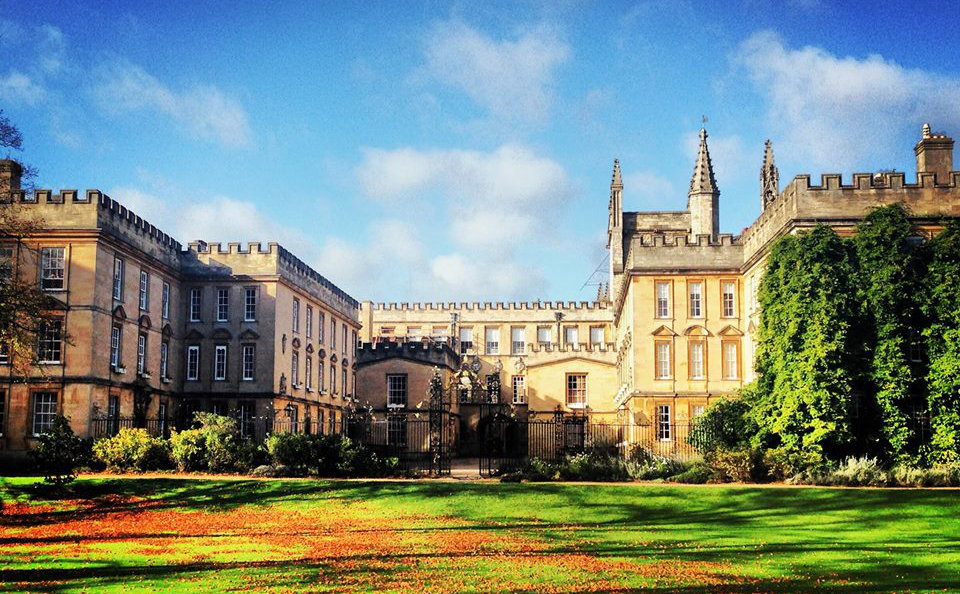
\includegraphics[width=\textwidth]{college.jpg}
                \caption[]{One of the nicer views
				of New College}
				\label{fig:college}
        \end{minipage}%
\end{figure}

\section{New College today}

New College is an intellectual community and one of the best-known colleges in
Oxford. New College has approximately 60~governing body fellows, 10~junior
fellows, 325 graduate students (109 freshers this year included),
420~undergraduates, an endowment of over \pounds160~million, a turnover of
\pounds13~million, and some of the most beautiful grounds and buildings in Oxford.

The college is governed, surprisingly, democratically, by the governing body
which consists of professorial fellows, tutorial fellows and a few others. New College has around 10~professorial fellows who hold university chairs. There are around 45~tutorial fellows who teach undergraduates in college as well as having university positions.

The primus inter pares is the Warden who serves as the figurehead of the college. Our current warden Sir Curtis Price is due to retire in August~2016, when he will be succeeded by Miles Young, who is currently Chairman and CEO of one of the world's largest communications groups, Ogilvy and Mather.

The fellows and senior college officers make up the senior common room, or SCR. Physically this is located between the Front and Garden quads. They dine to near Michelin star standard, have a wine cellar of 40,000~bottles and have luxurious offices in the Old Quad buildings.

The MCR is made up of graduate students, people reading for second undergraduate degrees, visiting students, a few post-doctoral researchers without a college allegiance, and 4th year undergraduates in sciences, languages, and some other subjects. Graduate students are primarily taught by the university, but have college as a social base and to provide additional resources.

The JCR, or junior common room, is the undergraduate body. They are taught between college,
where they have regular tutorials (hour long sessions with their tutors, individually or in pairs), and the university where they have lectures and practicals. Admission of undergraduates is the responsibility of the colleges.

New College is particularly famous for its musical and cultural education. It houses a world class choir, with associated choir school, and the fellows have written many of the world's leading textbooks in the discipline. New College has just received planning permission for a new music building, adjacent to the Victorian Savile House in Mansfield Road. The building, designed by John McAslan and Partners, will offer three floors of accommodation: the top floor will contain two chamber music studios; the first floor, four practice rooms; and the ground floor, a large rehearsal room for opera and drama. Work will begin during the summer of 2015.


\chapterimage{chapter_head_3i.jpg} % Chapter heading image

\chapter{People}
\addcontentsline{lof}{figure}{Chapter header \emph{Lantern}: Photo credit to
Kira Liebert}

\section{The MCR committee}

The MCR is run by a committee of students. Getting involved in the committee is great fun and a good way of being part of college life. You will hear more about how you can do this during freshers' fortnight. You can find the current MCR committee position holders and their blurbs on:
\url{http://mcr.new.ox.ac.uk/?n=Main.PeopleCommittee}

\noindent Please contact the committee with any queries. 

\noindent Our e-mail addresses can be found on the committee webpage above, or
by simply following the usual pattern of
\emph{\urlformat{firstname.lastname@new.ox.ac.uk}} (which is valid for most
members of the college).
If you are unsure of an e-mail address you can also search on
\url{www.ox.ac.uk/contact}.

\section{People in college}

\begin{description}

\item[The Warden]
The Warden is the head of college, and is ultimately responsible for all aspects of college life. 

From August 2016, this role will be taken by Mr Miles Young, who is the Chairman and CEO of one of the world's largest communications groups, Oglivy \& Mather.

The Warden lives in \emph{the Warden's lodgings}, accessed via the Front Quad.
He also has a private garden (\emph{the Warden's garden} - starting to get the
conventions?) which has amazing views of New College, Hertford College, and All Souls College.
Appointments to see the Warden can be made through the college secretary (\href{mailto:warden@new.ox.ac.uk}{\urlformat{warden@new.ox.ac.uk}}).

\item[Tutor for Graduates]
The Tutor for Graduates is a college fellow who, in addition to his or her academic duties, oversees the general well-being of the MCR within the New College community. The Tutor for Graduates also reviews each graduate student's termly reports, and negotiates with faculty supervisors and college advisers as appropriate. Additionally, he or she signs graduate applications for transfer or confirmation of status, and liaises with the Proctors, the University's regulatory officers, on the behalf of college members.

Graduate students may also draw on certain academic allowances, and the Tutor for Graduates reviews all these applications, as well as advises on scholarship possibilities. The Tutor for Graduates meets MCR committee members regularly over lunch to discuss academic and social life in the MCR, and also invites regular groups of graduates to High Table dinners, and hosts a couple of full MCR dinners in Hall each year. Finally, the Tutor for Graduates represents the MCR to the Governing Body, the sovereign body of college, which meets around three times a term. 

Any graduate who wishes to discuss their academic or social progress is referred to their college adviser in the first instance, but if you encounter any problems requiring more urgent attention, the Tutor for Graduates is always available. All enquiries concerning graduate matters should be directed to the College Office, which administrates for the Tutor for Graduates.

The Tutor for Graduates is currently Prof George Ratcliffe. A letter from him
welcoming you to New College was sent to you during the long vacation. You can
contact Professor Ratcliffe through 
\href{mailto:george.ratcliffe@new.ox.ac.uk}{\urlformat{george.ratcliffe@new.ox.ac.uk}}.

\item[Your College Advisor]
The Tutor for Graduates assigns each graduate student an academic advisor in college, typically a college fellow who works in the subject area of their advisee, but who is not their advisee's main supervisor. Your advisor is supposed to be your first port of call if you have any academic difficulties on which you would like an independent opinion.

Your advisor should contact you during your first term via your Oxford email address. The purpose of this contact is purely to touch base and ensure your transition to Oxford is proceeding smoothly. You are also encouraged to make contact with them. If you have any problems with your adviser please contact either the MCR President or the Tutor for Graduates.

\item[Bursar]
The Bursar, David Palfreyman, is responsible for the college's finances. If you have any unforeseeable financial difficulties he may be able to help you. Appointments to see him should be made through his secretary, either by going to the Bursar's Office (4OB1) or by emailing \href{mailto:bursar@new.ox.ac.uk}{\urlformat{bursar@new.ox.ac.uk}}.

\item[Home Bursar]
The Home Bursar, Caroline Thomas, is responsible for the domestic side of college life, including accommodation, college staff, and food. She is also part of the welfare team. Contact her either by e-mail (\href{mailto:caroline.thomes@new.ox.ac.uk}{\urlformat{caroline.thomes@new.ox.ac.uk}}) or in the Home Bursary on the ground floor of 4OB.

\item[Dean]
The Dean, Dr Michael Burden, is responsible for discipline in college. Day-to-day running of this side is carried out by the Assistant Dean and three Junior Deans. If you want to hold an event in college, you have to apply to the Assistant Dean for permission. Hopefully, this is the only time you will have to see the decanal team!

\item[IT Officer]
James Dore is the college's IT Officer. His team is responsible for the computer provision in college. They are available to deal with any computer related issues you may have. They have an office in the Garden Quad (12OB-2) and can also be reached through
\href{mailto:it-support@new.ox.ac.uk}{\urlformat{it-support@new.ox.ac.uk}}

\item[Welfare Fellows (Cox/Salvesen Fellows)]
College employs two Junior Research Fellows who also have a welfare role; they
are called the \emph{Cox and Salvesen Fellows}. They are currently Sarah Crook (\href{mailto:sarah.crook@new.ox.ac.uk}{\urlformat{sarah.crook@new.ox.ac.uk}}) and Ryan Hanley (\href{mailto:ryan.hanley@new.ox.ac.uk}{\urlformat{ryan.hanley@new.ox.ac.uk}}), respectively.


\item[Porters]
The Porters live in the lodge in the Holywell Quad (there is also a lodge at the sports ground) and are the first port of call for all everyday issues in college, e.g. lost keys, light bulbs, etc. The Porters work long hours and deal with all the various and quirky needs of college members. Please be polite and friendly when dealing with staff at either lodge.
\end{description}


\chapterimage{chapter_head_4.jpg} % Chapter heading image

\chapter{Facilities}
\addcontentsline{lof}{figure}{Chapter header \emph{Branches}: Photo credit to
Kira Liebert}
\addtocontents{lof}{\protect\vspace{\baselineskip}}
 
\section{New College}

\subsection{The MCR - The Rew Nooner Spoom}\label{ssec:Spoom}

This is your common room - the actual MCR. It was named after the Rev. Spooner, Warden of New College from 1903-1924, who was famous for his verbal gags or \emph{Spoonerisms}: hence the name. The MCR is commonly called \emph{the Spoom}. It is accessible 24 hours a day and has a 42'' television, Nintendo Wii, PS4 (doubling as BD/DVD-player), board games, books, coffee machine, wi-fi, and newspapers as well as other publications. The TV somes equiped with Netflix and a wide range of TV channels including Sky Movie, Sky Atlantic, Sky Sports, BT Spotrs and ESPN. It also has a bar area which is opened regularly - usually on Wednesday and Thursday nights during term time, as well as after guest night dinners. It is also used for other purposes, including a free brunch each Sunday morning during term time.

Since 2009, the Spoom has been located in the Weston Sports Pavilion.
Refurbished recently, the Rew Nooner Spoom (New Spooner Room) is undoubtedly one
of the most comfortable and inviting MCRs in Oxford. The facilities are split
across the main living room area upstairs and the television and computer room
downstairs, which also has a small library.
Access to these rooms and indeed the Sports Pavilion is since 2013 by your
bod-card. If you are confronted with any bod-card malfunction issues, contact
either Lauren Burton (\href{mailto:lauren.burton@new.ox.ac.uk}{\urlformat{lauren.burton@new.ox.ac.uk}}), or the deputy clerk of works, Chris Conway (\href{mailto:chris.conway@new.ox.ac.uk}{\urlformat{chris.conway@new.ox.ac.uk}}).

\begin{figure}[htbp]
\centering
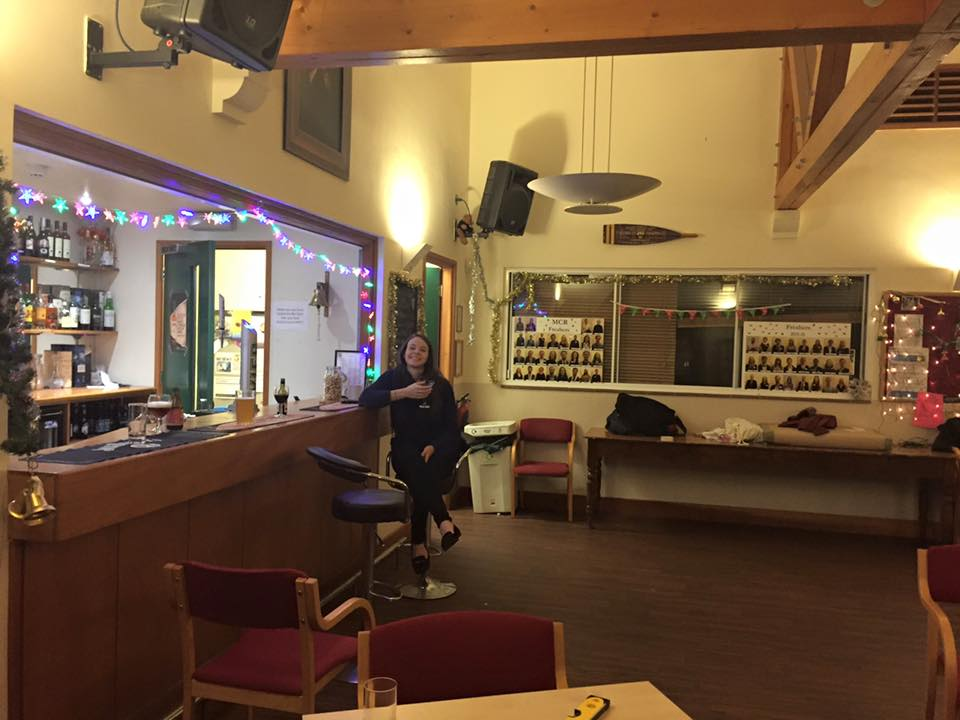
\includegraphics[width=0.85\textwidth]{Spoom.jpg}
\caption[]{The Rew Nooner Spoom}
\label{fig:Spoom}
\end{figure}

\subsection{The JCR}

Graduate students are also members of the Junior Common Room (primarily the undergraduate body of college). The physical JCR is located in the Garden Quad and has a satellite television, pool table and games consoles. There are also a few computers that can be access with New College credentials.
\subsection{Hall}

\emph{Hall} refers to the dining hall in college. The Hall is located in the oldest
part of college with the buttery next to it. Food is available to graduates during term time; all meals are charged to your till account and paid for using your Bod-card (see below). 

\smallskip

\begin{description}
\item[Breakfast:] Breakfast is available from 8\,am to 9\,am on weekdays
and 11\,am to 1\,pm at weekends. A choice of an \emph{English} cooked breakfast,
\emph{continental} breakfast, cereal etc. is available and charged per item, for
a total of about \pounds1.50-\pounds2.00.
\item[Lunch:] Lunch is available 12\,am to 1.30\,pm on weekdays. Lunch can be
charged per item individually, a meal consisting of main, potatoes, veg and
salad will be charged at \pounds3.50.
\item[Dinner:] 
Dinner comes in two sittings, early and late, usually referred to as \emph{informal
hall} and  \emph{formal hall} respectively. As of
October 2014, evening meals cost \pounds6.26 inclusive of soup, salads, a main
course, potatoes/pasta, vegetables, and dessert. Students MUST book their meals before
10\,am on the day they want to go to dinner in the Hall. This is done on-line at
\url{http://food.new.ox.ac.uk/}, where you also have to specify the sitting you
wish to attend.

Informal hall is available every day, canteen style, and food can be bought
between 5:45\,pm to 7:00\,pm (6:30\,pm on Fridays). 

Formal hall is held every Tuesday, Thursday and
Sunday during term time, and is served. For formal hall diners
have to be seated for 7.15\,pm, stand when the Fellows enter, then sit after
saying grace. Unusually for Oxford, we do not stand up when the Fellows leave
at the end of dinner. During these dinner we have to wear gowns, but can wear
them over casual clothing.

There are occasionally other dinners, in particular guest night dinners, which
are held fortnightly on odd-numbered term weeks. These guest dinners are a great
favourite of the MCR for their lavish 3-course catering and the customary
after-parties. One great perk of New College dinning is that MCR members may
bring up to 4~guests. Guest night dinners are charged at \pounds~15.55 per
person.

\item[Dining on high table:] Fresher graduates may dine at high table once
during their first year with the Tutor for Graduates (if they reply fast enough
to the invitation emails).
This will be advertised during term. You could also try and persuade your college adviser to invite you to dine at high table.
\end{description}

\subsection{College Bar}
The college bar, beer cellar, or JCR bar, is primarily college run. It is open
all day offering sandwiches, cakes, coffee and beverages and starts serving
alcohol from 6\,pm to 11\,pm during term, and often out of term as well. The bar
is located under the hall and has games such as table football.

Drinks are cheap (considerably cheaper than in town), and priced at the
level of the MCR bar. You can pay cash but it is slightly cheaper to use your Bod-card and charge it to your till account.

\subsection{Sports facilities}
New College has one of the best and most beautiful sports grounds in Oxford, located a five-minute walk from college on St. Cross Road. This has football and rugby pitches, a cricket pitch and nets, one hard tennis court and six grass courts and a volleyball court in the summer. There is a squash court and table-tennis table in the pavilion. Many of the facilities can be in the Weston lodge or using the online booking system. There is plenty of equipment in the Weston lodge for many of these sports for use by MCR members. 

College has sports teams in a wide range of sports: details will be available during freshers' fortnight. The collegiate nature of the university makes it very easy to get involved in sport whilst at Oxford.

Rowing is very popular in Oxford. College has a boathouse on the Isis and a very active boat club. There will be several novice boats run during Michaelmas, as well as opportunities for experienced rowers. Again, these will be advertised in freshers' fortnight.

We also have a punt shed located at the sports ground; punts may be taken out
from here during the summer. New College does not have its own gym. However,
members of college have free access to the university gym at the Iffley Road. To
access the Iffley Road gym, simply bring your Bod card to the gym's front desk
and inform the attendant of your college membership. You will be asked to fill
out some paperwork. Another work-out option is the University Club, which is
very close to New College on Mansfield Road, and of which all Oxford graduate
students are members. A year-round pass to the Club's gym may be purchased for
around \pounds60.

\begin{figure}[htbp]
\centering
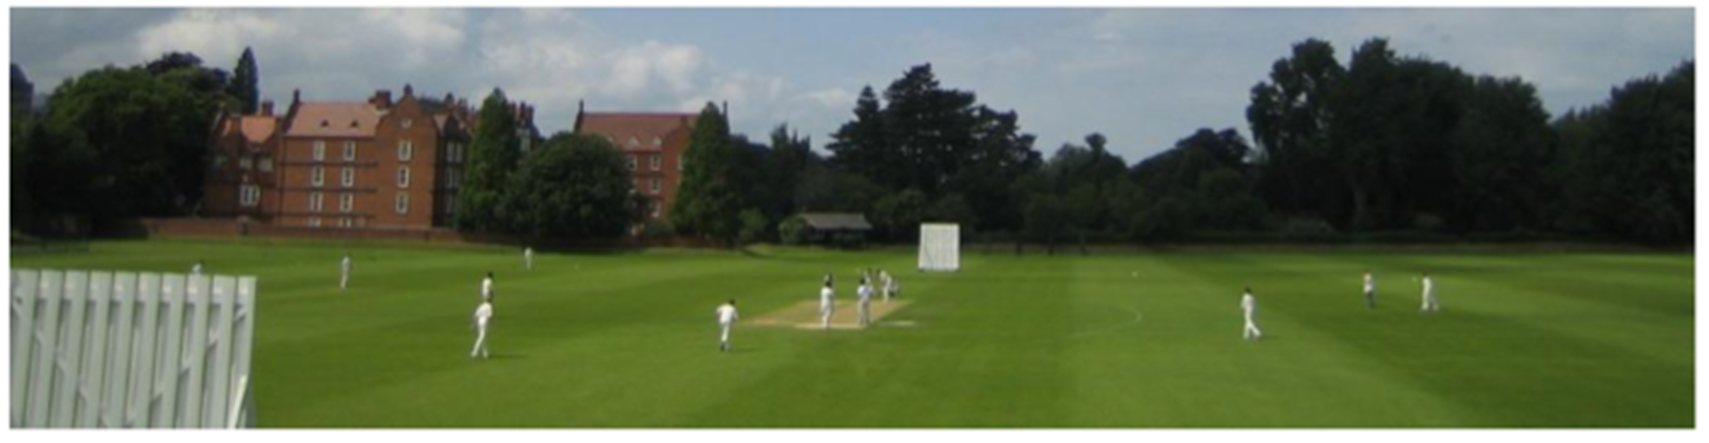
\includegraphics[width=0.9\textwidth]{sports.png}
\caption[]{The College sports ground}
\label{fig:sports}
\end{figure}

\subsection{MCR BBQ}
In 2013 we had a communal BBQ built behind the cricket pavilion overlooking the sports ground. It is currently available for MCR events only, but is intended to be accessible for any MCR member's private function in the future. The MCR committee usually organizes BBQ-related events in the end of Trinity term and during the summer break.
\subsection{The Library}
The College has a library which is located in the Holywell Quad. It is open from
8.30\,am to midnight during term and from 08.30-17.00 out of term (the student body is campaigning hard to lengthen these hours). The library's collection is aimed mainly at undergraduate studies; however, the library is also available for graduates to use for work. Books and DVDs may be borrowed from the College library.
\subsection{IT}
All rooms in college have ethernet access. This connection can be activated by plugging in your computer using an ethernet cable, opening your internet browser and following the automated security program. There is also wi-fi in the Spoom, Weston buildings, JCR and library which is activated in the same way. Returning students should  find that wi-fi coverage has now improved with reasonable signal reaching even the upstairs rooms. IT services are continually working to improve wireless internet connectivity throughout the college. 

There is an MCR computer room in the Sports Pavilion containing two PCs and a laser printer. There is also a JCR computer room in NB2, which has some more advanced printers. Printing is charged to your Battels. 

All college members will have a college e-mail address. Your address will be in the
form \emph{\nolinkurl{firstname.surname@new.ox.ac.uk}}. You will almost
certainly have a second one in your department but (with a few exceptions) they all go to the same account.
There will be details of how to set up your account in your pidge soon after you
arrive. There is a webmail interface, but the account is easy to configure for
an e-mail client. See: \url{http://www.oucs.ox.ac.uk/email/config/}

\subsection{Chapel}
The chapel welcomes all college members to its services, which take place during the eight weeks of university term. We hope the chapel will be a place where anyone can find community, inspiration in words and music, and calm during busy weeks. Services follow the pattern of the Anglican church: the music is sung by the chapel choir, which has an international reputation, and the liturgy is formal to fit in with the building and the music, but aims to be as inclusive as possible and to focus on issues in the wider world. Any college member is welcome to get involved in chapel life - as readers, servers, and chapel wardens.

Services are held every weekday evening apart from Wednesday. College communion is at 9\,am on Sunday and is followed by breakfast. Advent and Christmas Carol Services are held on the Sundays of 8th week and 9th week of Michaelmas Term.

The beautiful chapel is also close to the scenic cloisters, a favourite spot of many for its peaceful, shaded ambience. The scene in Harry Potter and the Goblet of Fire where Draco Malfoy is turned into a ferret was filmed in the cloisters here. 

All information about the chapel may be found on the termly chapel card copies
in pigeon holes and on the chapel and lodge notice boards and on the chapel page
of the college website, and the choir website (\url{www.newcollegechoir.com}).

\subsection{The Gardens}
New College has some beautiful gardens, which are the responsibility of the Garden Fellow, Robin Lane Fox. Nobody is permitted to walk on the grass in the Front Quad, but all other areas may be used by students. Croquet may be played in the Holywell Quad, but no other ball games are allowed.
The main gardens are surrounded by the city walls and contain a decorative
\emph{Mound}. Do not climb, or let your guests climb, the city walls: this is an
offence, not just at college, but also at university level and the punishment is to be sent down.

\subsection{Chalet}

During your time at New College, please take advantage of our chalet in the
French Alps. With Balliol College and University College, we share an historic
property near Mont Blanc, which in 2009 celebrated its 100th birthday following
its reconstruction after the original 1865 chalet was accidentally burnt down in
1906. Each summer, two or three groups from New College spend 10~days reading
and walking in one of the most beautiful parts of Europe. All members of the college are welcome.
Groups are normally a mix of undergraduates and postgraduates with a few members
of the SCR. The trip is very inexpensive (usually less than \pounds5 per day), and
travel by air through Geneva or on the sleeper train from Paris is easy. For
more information, please consult the college page on the chalet
(\url{http://www.new.ox.ac.uk/new-college-chalet}).

\begin{figure}[htbp]
\centering
		\begin{minipage}{0.3\textwidth}
                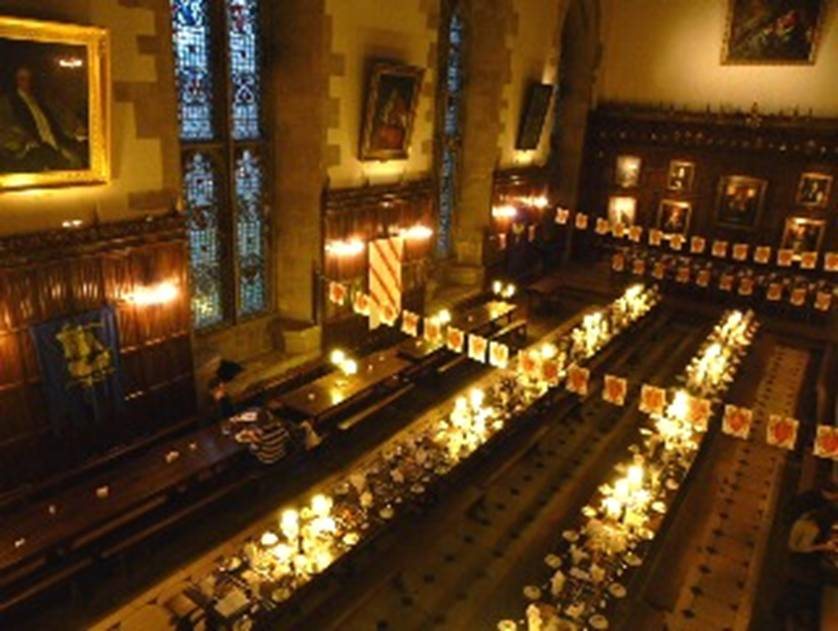
\includegraphics[width=\textwidth]{hall.jpg}
                \caption[Hall: Photo credit to Maureen Lenker]{The hall, set for
                a medieval dinner}
                \label{fig:hall}
        \end{minipage}%
        \quad
        \begin{minipage}{0.33\textwidth}
                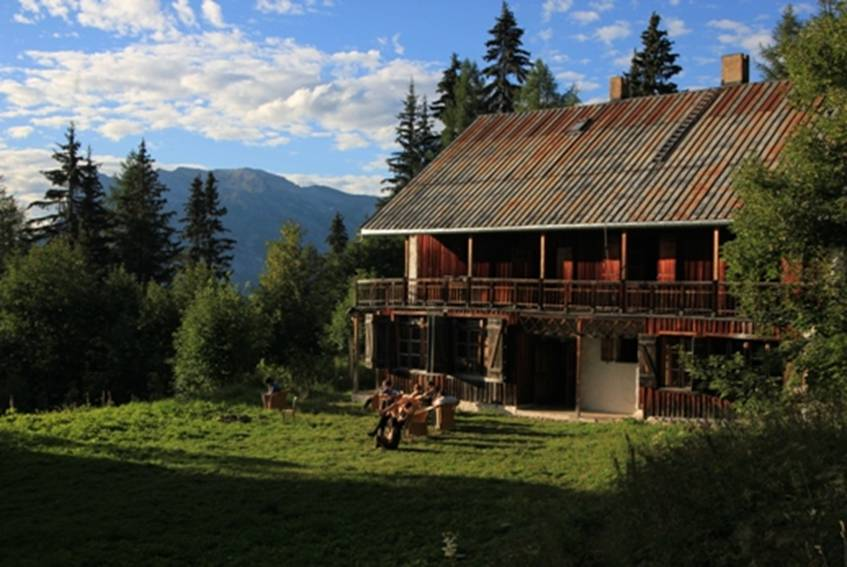
\includegraphics[width=\textwidth]{chalet.jpg}
                \caption[Chalet: Photo credit to Nick Altemose]{The
                \emph{cha\-let des ang\-lais}}
                \label{fig:chalet}
        \end{minipage}%
        \quad
        \begin{minipage}{0.3\textwidth}
                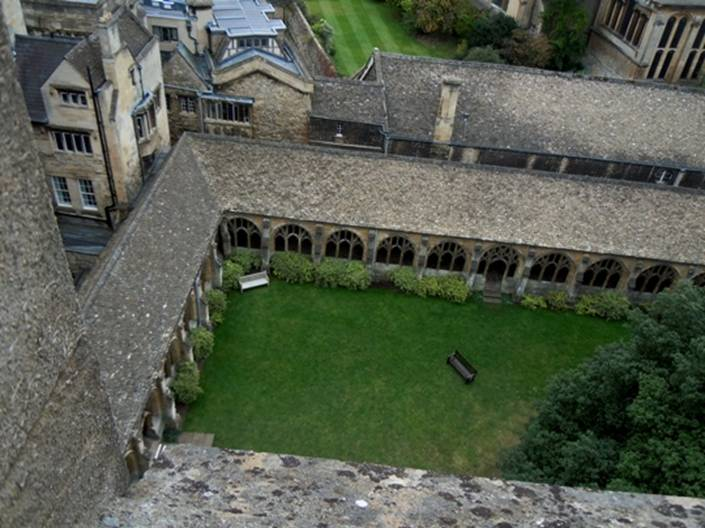
\includegraphics[width=\textwidth]{clois.jpg}
                \caption[Cloisters: Photo credit to Alex Graham]{The cloisters
                from New College tower}
                \label{fig:clois}
        \end{minipage}%
\end{figure}

\subsection{Pigeon hole}

You will be given a pigeon hole, referred to as your \emph{pidge}, in the post
room by the porters' lodge. This is where you collect your mail, both internal and external. Your address will be: Yourname,~New College,~Holywell~Street,~Oxford,~OX1~3BN,~UK.

You can send post internally across the university by dropping it in at the porters' lodge. There is a postbox for external mail under the Holywell arch and the closest place to buy stamps is the Tuck Shop on Holywell Street.

\section{The University}

\subsection{Libraries}
Oxford has numerous different libraries. As a student, you are a reader at the
famous Bodleian and the associated Radcliffe Science Library. There will also be
a library in your department. Most of the academic libraries in Oxford are part of the Bodleian Libraries system. See: \url{http://www.bodleian.ox.ac.uk/}.

\subsection{Sports facilities}
The University's main sports facilities are located a 10~minute walk from
college on Iffley Road. This site has a gym (free to New College students, excellent swimming pool (\pounds82/year), running track (where Roger Bannister ran the first four minute mile), tennis courts, squash courts, sports hall, indoor cricket nets and a number of other facilities.

There is also a wide range of university sports teams. Find out about these
either online (\url{www.sport.ox.ac.uk}) or sign-up at the freshers' fair during
freshers' week.
\subsection{Students union - OUSU}
Oxford students are also represented by the student union. This has its
headquarters in Bonn Square. They are a useful source of information on a number
of topics; check \url{www.ousu.org} for more information.
\subsection{The Oxford Union}
Although not officially part of the university, the Oxford Union is closely
associated with it. The membership fee in 2013 was \pounds236, or \pounds213 during freshers'
week, but is for life. However, the Union runs many good events, attracts many
famous speakers and are one of the leading debating societies in the world. During freshers' fortnight it is open to all, so check it out then even if you do not choose to join. The building is on St. Michael's Street. See: \url{http://www.oxford-union.org/}
\subsection{The University Club}
The University Club is open to all graduate students and staff of the
university. It is located near to New College on Mansfield Road. The good news
is that basic membership is free. It has a bar, lots of screens to watch sport
on, gym facilities, a small astro-turf and a playing field. It also has football and cricket teams which several New College graduate students are involved in. See: \url{www.club.ox.ac.uk}
\subsection{The Careers Service}
The University Careers Service, located at 56~Banbury Road, is the main resource
for what happens after you leave Oxford. Whether it is landing an internship or
job, applying for postgraduate study or a postdoc anywhere in the world, or just going to a Careers Fair to get free stuff, it is recommended to register with them on their website: \url{www.careers.ox.ac.uk} to be able to access the range of advice and information. The Director of the Careers Service, incidentally, is a member of the New College SCR (Jonathan Black).

\section{Town}
Oxford has a large non-student population and there is a lot going on outside of
the university. The following list barely scratches the surface of what you can
do. \url{www.dailyinfo.co.uk} is a good source of information on what is going
on around the city.
\subsection{Sporting clubs}
As well as University clubs, there are many town sports clubs, i.e. not part of the university. These are often more expensive than university clubs, but some have better facilities and they will have a different atmosphere. Many graduate students use gym facilities which are not part of the university.
\subsection{Pubs and bars}
Oxford has a fantastic selection of pubs and bars. Sadly, with the notable
exception of the King's Arms, few pubs are open past 11\,pm (the traditional
closing time for pubs in the UK). The MCR committee will do its best to familiarise you with some of these during freshers' fortnight.
\subsection{Clubs}
There are also some nightclubs in Oxford. Many of these are very student-centric during term-time. London is also only an hour away and there are excellent bus and train links.
\section{Doctors}
Occasionally we all get ill and need to go visit the doctors. During term and out of term the doctors can be found in their practice on Beaumont Street. Your medical registration will occur during the 1st week of Michaelmas term, after which you will have access to the College doctors. Information about the registration procedure will be given by the college during the freshers’ week. 

The following information on going to the doctors has been taken from the
college website: \mbox{\url{http://www.new.ox.ac.uk/medical}}.

The College Medical Officers, (College Doctors) Dr John Sichel and Dr Clare
Stephenson have agreed to accept any member of the College who is resident in
the UK for longer than 6~months as an NHS patient. Their practice is at 28~Beaumont Street (01865~311811; \url{www.28beaumontstreet.co.uk}), and they hold
a surgery in College in 1~NB in term times.


\subsection{Overseas students and visiting students}
All overseas students who are studying here for more than 6~months can register
and have access to the UK National Health Services (NHS). In order to do that,
the students must register with the College doctors. It is particularly
important that overseas students register with the College doctor {\textbf{as soon as possible}}. Please note: you will not be able to register if you have less than 6~months of your course left.
Visiting students on courses longer than 6~months are eligible for NHS treatment (please see above for details). Those in Oxford for a course less than 6~months (in effect, less than 3~terms of study) will not be eligible for medical treatment under the NHS, and are required to make arrangements for private medical insurance before arriving in the UK.
You should make an appointment to see the College Doctor, who may be able to offer special private terms, but will be unable to offer consultation or treatment within the National Health Service unless your usual country of  residence has a reciprocal health agreement with the UK.
For more information on charges for NHS treatment and exemptions for people
visiting the UK, see the Department of Health's website for
\href{http://www.nhs.uk/chq/pages/1086.aspx?categoryid=68}{overseas visitors}.
There are two NHS dentists that are known to take on students: Studental (located at Oxford Brookes University in Headington; telephone: 01865~484068, e-mail: \href{mailto:reception@studental.co.uk}{\urlformat{reception@studental.co.uk}}) and Oasis (22 Beaumont Street, Oxford, OX1 2NA; telephone: 01865~243702, e-mail: \href{mailto:reception.oxford@oasis-healthcare.com}{\urlformat{reception.oxford@oasis-healthcare.com}}).


\chapterimage{chapter_head_1.jpg} % Chapter heading image

\chapter{What the MCR does for you}

\section{Freshers' Fortnight}
One of the most important things that the MCR does is to provide two weeks of
entertainment and orientation for you when you arrive. Details will be published
when you arrive (both in your pidge and posted around accommodation). The first
event will be held in the Spoom\ref{ssec:Spoom} on Sunday of 0th week (4th
October).
This will be followed by a wide range of events: parties, dinners, pub crawls, quizzes, teas and many more events to help you settle in. It all finishes with the matriculation ceremony on Saturday of 1st week when you formally become part of the University. You do not need to matriculate if you have already studied at Oxford, Cambridge, or Trinity College, Dublin. Remember to wear your sub-fusc and gown to matriculation!

\section{Guest night}
Our main regular social events are \emph{guest nights}. MCR guest nights happen
on Friday of odd weeks so there are four a term. Dinner is usually of a very
high standard and costs \pounds15.55. Members may invite up to four guests to
join them, although many prefer to enjoy the evening with friends from college. Dress is smart, but gowns are not required. After dinner, there are second desserts provided by the MCR which include a selection of cheeses, fruit, chocolate and port, as well as the bar being open. Everyone is welcome to come to this even if you didn't attend the dinner.

Guest nights are very popular and you need to sign-up early on
\url{food.new.ox.ac.uk} to avoid disappointment. Sign-ups start a week early: at
12:01\,am on the preceding Friday.

\section{End-of-term dinners}
The last guest night of term is an end-of-term dinner for which the MCR puts up
a subsidy to make this last dinner extra special. Guests are limited to allow as
many MCR members as possible to attend. Expect a theme, decorations, free drinks and an after-party with a DJ in the MCR.
\enlargethispage{\baselineskip} %Widow avoidance

\section{End-of-year garden party} 
At the end of Trinity term the MCR holds and end-of-year party to say goodbye to the many people leaving Oxford. Enjoy a bouncy castle, games, Pimm's and other summer delights taking you from the day to dancing at night, and pray for good weather! 

\section{Exchange dinners}
We have \emph{exchanges} with other colleges, whereby we host them at New
College for drinks and dinner and then they do the same for us. Drinks and second desserts are included. These events vary between being a special dinner with high table food or occurring during regular formal dinners. The MCR also tries to do an exchange with a Cambridge college once a year. 

\section{Brunch}
During term, and occasionally out of term, the MCR hosts a free brunch in the
Spoom on Sunday mornings at 11\,am. This is a good way to catch up with friends and meet new people. Arrive early to avoid missing out on the smoked salmon!

\begin{figure}[htbp]
\centering
		\begin{minipage}{0.45\textwidth}
			\centering
				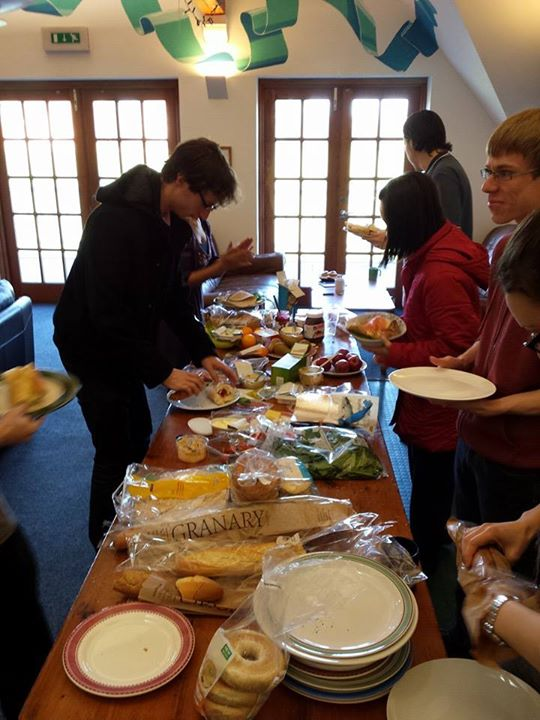
\includegraphics[width=0.9\textwidth]{brunch.jpg}
				\caption[]{A brunch in the Spoom}
                \label{fig:brunch}
        \end{minipage}%
        \quad
        \begin{minipage}{0.45\textwidth}
        	\centering
				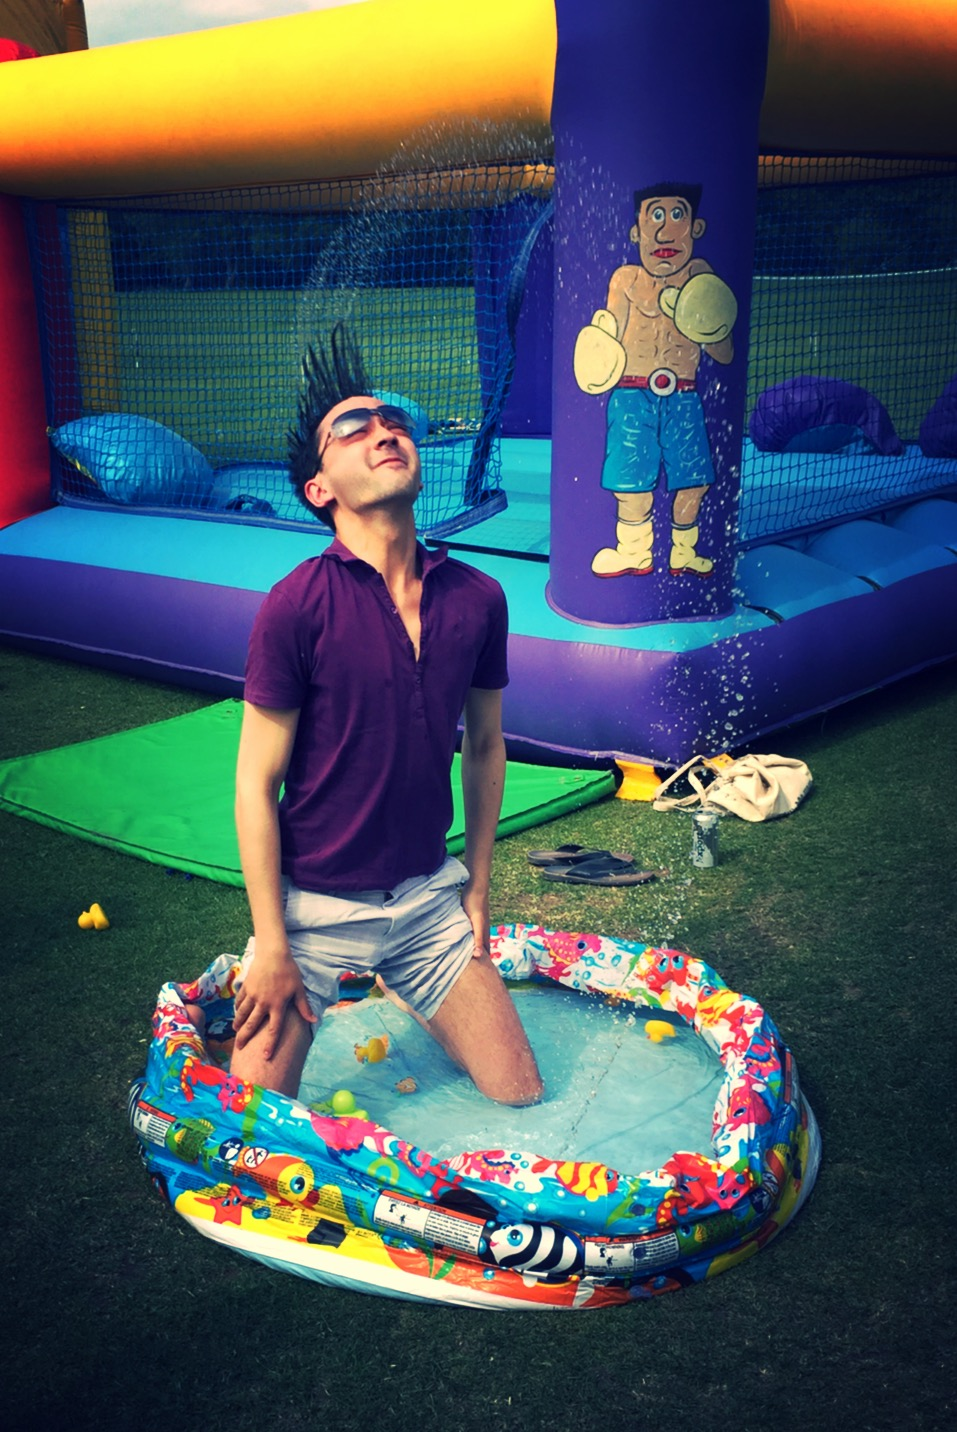
\includegraphics[width=0.9\textwidth]{eoyp.jpg}
				\caption[]{Typical scene at the
				garden party}
				\label{fig:eoyp}
        \end{minipage}%
\end{figure}

\section{Bar Nights}
During term the MCR opens the bar between 9.00-11.00\,pm on a Wednesday and
Thursday. The bar is also open on alternate Friday evenings and the occasional Saturday evening.


\begin{figure}[htbp]
\centering
		\begin{minipage}{0.45\textwidth}
				\centering
				
\includegraphics[width=.8\textwidth]{bar.jpg}
				\caption[]{Absolutely typical bar night}
				\label{fig:bar}
        \end{minipage}%
        \quad
        \begin{minipage}{0.45\textwidth}
				\centering
				\includegraphics[width=.8\textwidth]{bop.jpg}
				\caption[]{A bop}
				\label{fig:bop}
        \end{minipage}%
\end{figure}

\section{Bops}
Bops are the highlight of the MCR party scene. Around once a term the MCR will
throw parties with a fun theme and a DJ in the Spoom. They normally occur after guest night dinners and the bar remains open later than usual. Other colleges also host their own Bops located on their grounds, which you are welcome to attend if advertised. 

\section{New Collection}
The MCR's own multi-disciplinary academic journal, The New Collection, aims to present the breadth and depth of work currently being undertaken by the graduate members of New College. All work contained within the journal is by current graduate MCR members and every MCR member is encouraged to get involved by either submitting an article or during the editorial phase.

The New Collection provides members the unique opportunity of learning both how to write and review journal articles all within the supportive structure of New College, making us the envy of other colleges. Successful articles this year came from a variety of disciplines and were aimed at a broad readership, which is the original aim of the New Collection - to bring the current work of our MCR members to a larger intellectual audience.

\section{Colloquia}
Each term, members of the MCR are invited to present their research in colloquia. Around 2009, we introduced a new tradition, collaborating with the SCR for the first time. The colloquia comprise a 20-30 minute talk by a graduate student, followed by a response from a member of the SCR working in the same field. The floor is then opened to general questions and discussion, with members from not just the MCR, but also JCR and SCR invited to attend. These talks are an excellent opportunity to gain presentation experience, but more importantly the Graduate Colloquia are the cornerstone of our intellectual engagement with College. The atmosphere is informal and supportive, and offers a chance to learn what it is your peers may be working on in labs and libraries when away from Weston and the Spoom! The new SCR involvement also offers a great chance to get expert feedback on your work from someone other than your supervisor. Past colloquia have covered topics ranging from The Universe, to Crime fiction. The goal is to present an academic topic in which you are presently immersed to an audience who may or may not have experience of the concepts.

The MCR Vice-President organizes the colloquia and is always seeking MCR members
willing to present a colloquium, so please consider doing so, emailing Tanja
Collavo
(\href{mailto:tanja.collavo@new.ox.ac.uk}{\urlformat{tanja.collavo@new.ox.ac.uk}})
if you are interested.

Since last year, a fervour forum has been introduced as well, always organized
by the MCR Vice-President The Fervour Forum consists of 5\,minutes
presentations/demonstrations of an MCR member's hobby or passion and followed by 5-10 minutes Q\&A. Usually there are 3-4 presentations in the same way and they represent a great way to know better other MCR members and learn new, funny and interesting things.

\section{The MCR play}
The Arts and Culture organizes every year a theatre played performed in Trinity
term either in the college garden or cloisters. Actors and Production team are
selected primarily from volunteers from the MCR. The play is usually on stage for an entire weekend and requires around six weeks of preparation and rehearsals. In 2015 the MCR produced Hay Fever, a comedy set in the '20s, obtaining a great success across both college and non-college audiences. If you want to be involved with the next MCR theatre play, get in touch with Dionysios (\href{mailto:dionysios.kyropoulos@music.ox.ac.uk}{\urlformat{dionysios.kyropoulos@music.ox.ac.uk}}).

\begin{figure}[htbp]
\centering
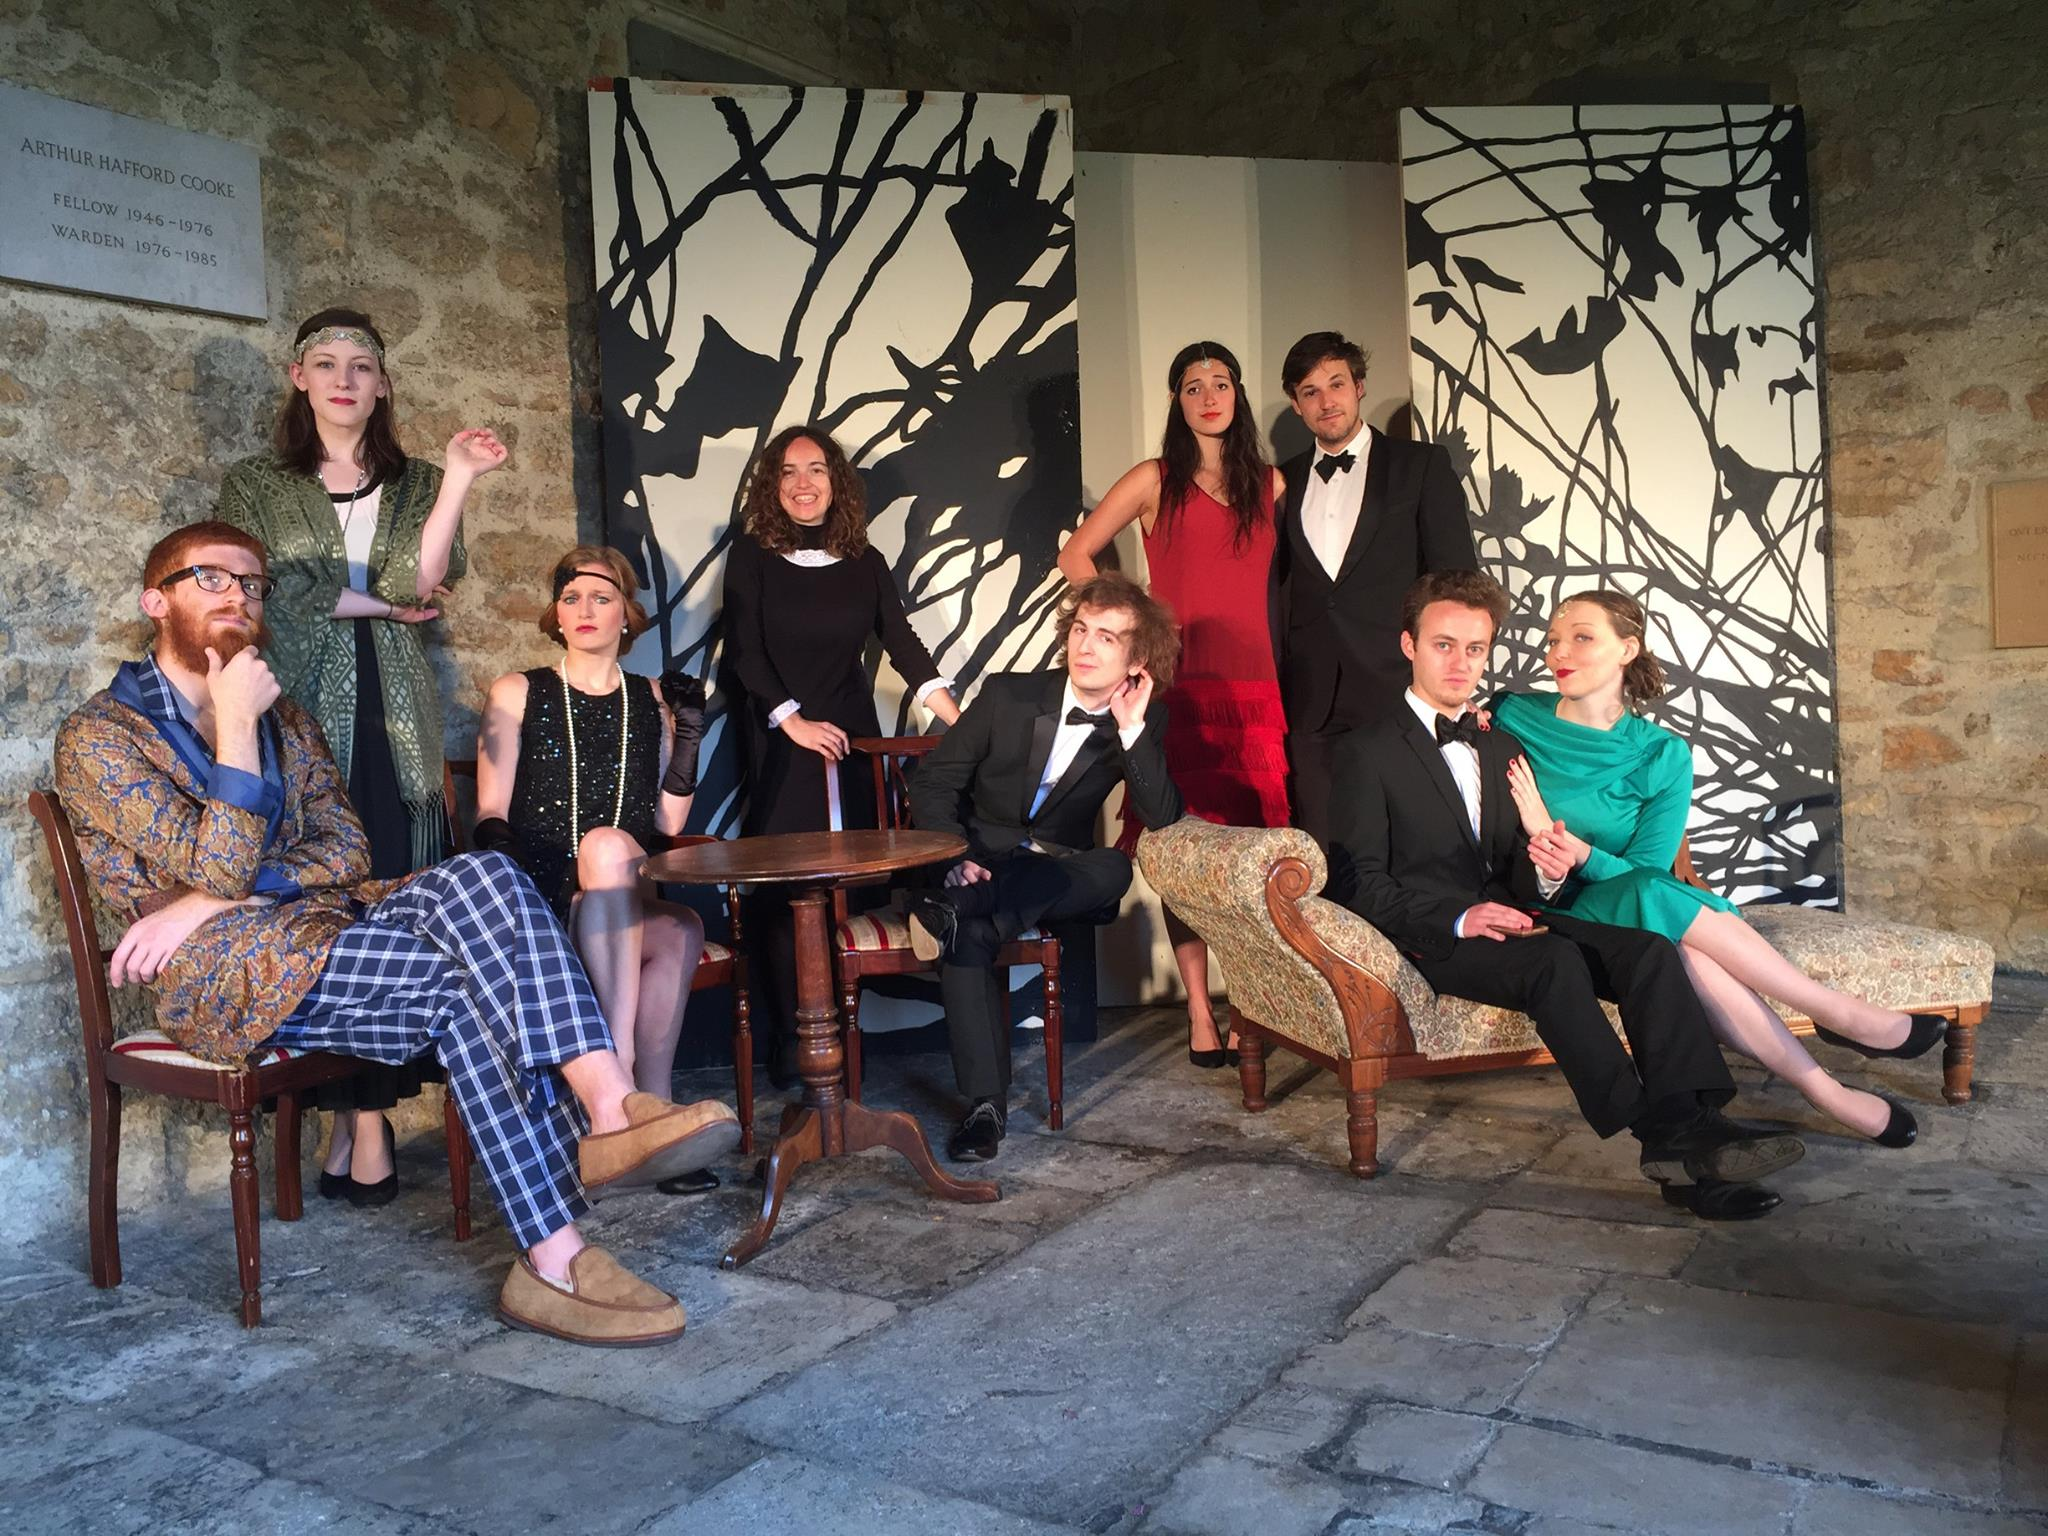
\includegraphics[width=0.75\textwidth]{play.jpg}
\caption[]{The 2015 MCR play,
\emph{Hay Fever}}
\label{fig:play}
\end{figure}

\section{Other events}
The MCR puts on several other events during the term in addition to the regulars. These include orchestral concert trips, MCR quizzes, a play, cheese and wine tasting, etc. These occur regularly throughout term, so keep an eye on the MCR mailing list and Facebook page for adverts.


\begin{figure}[htbp]
\centering
		\begin{minipage}{0.3\textwidth}
                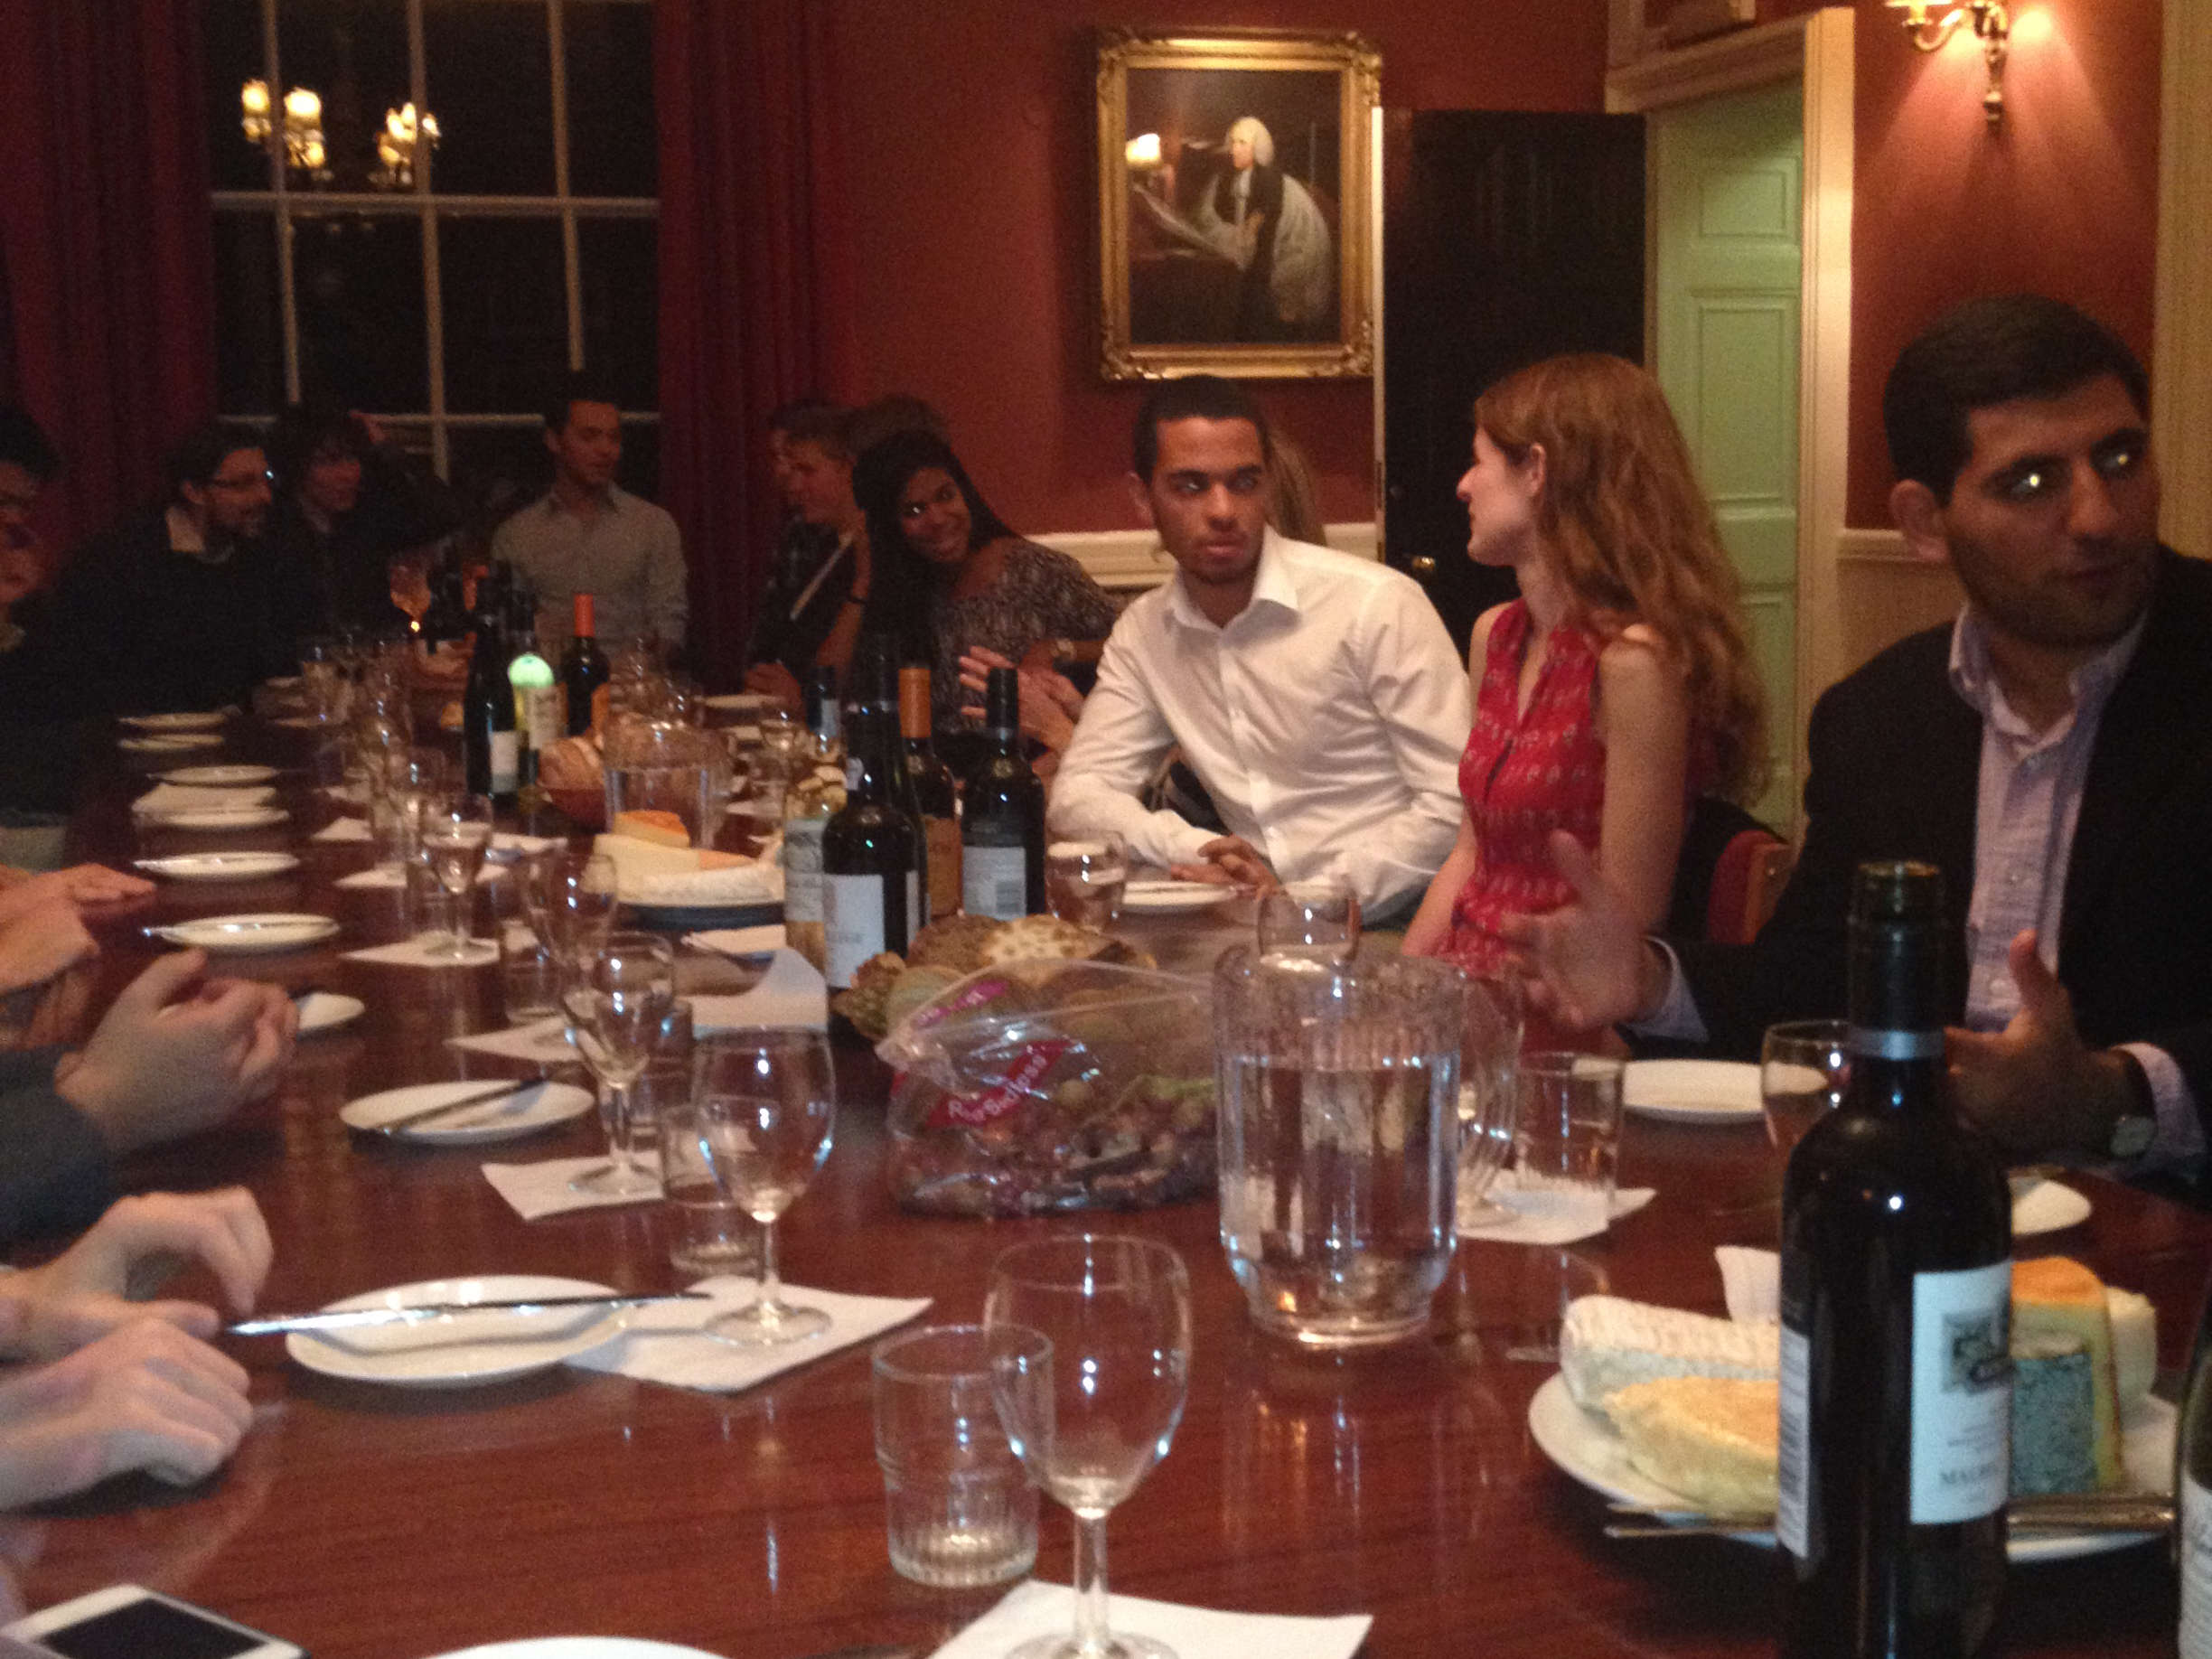
\includegraphics[width=\textwidth]{cheese2.jpg}
                \caption[]{Cheese and Wine tasting}
                \label{fig:cheese}
        \end{minipage}%
        \quad
        \begin{minipage}{0.3\textwidth}
                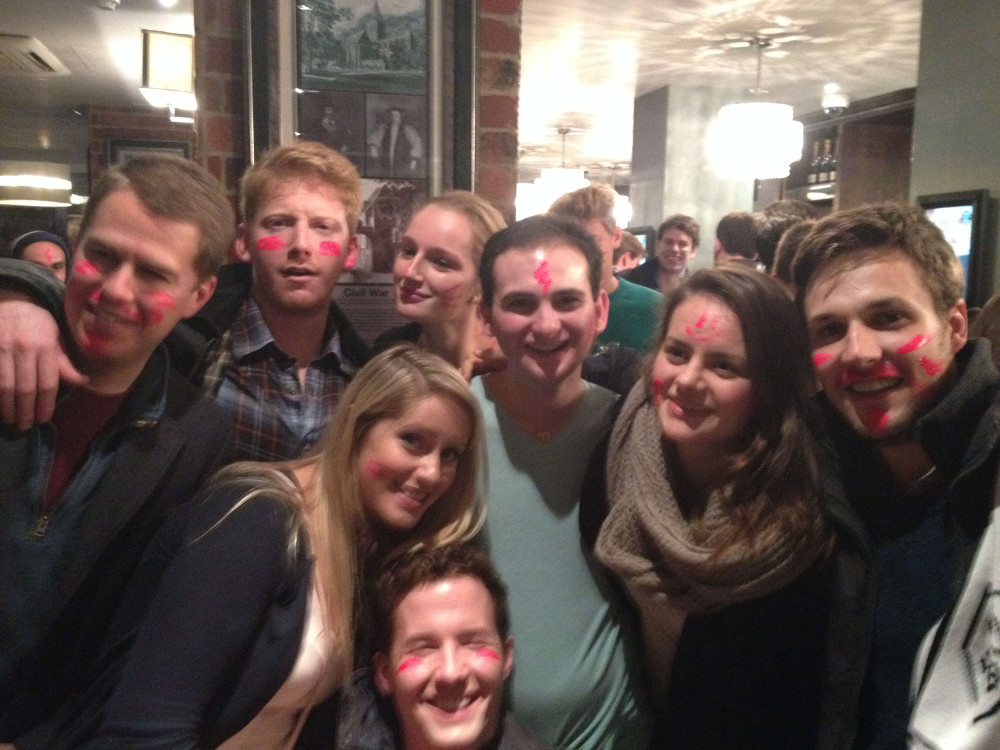
\includegraphics[width= \textwidth]{pub.jpg}
                \caption[]{Freshers' Week Pub Crawl}
                \label{fig:crawl}
        \end{minipage}%
        \quad
        \begin{minipage}{0.30\textwidth}      
                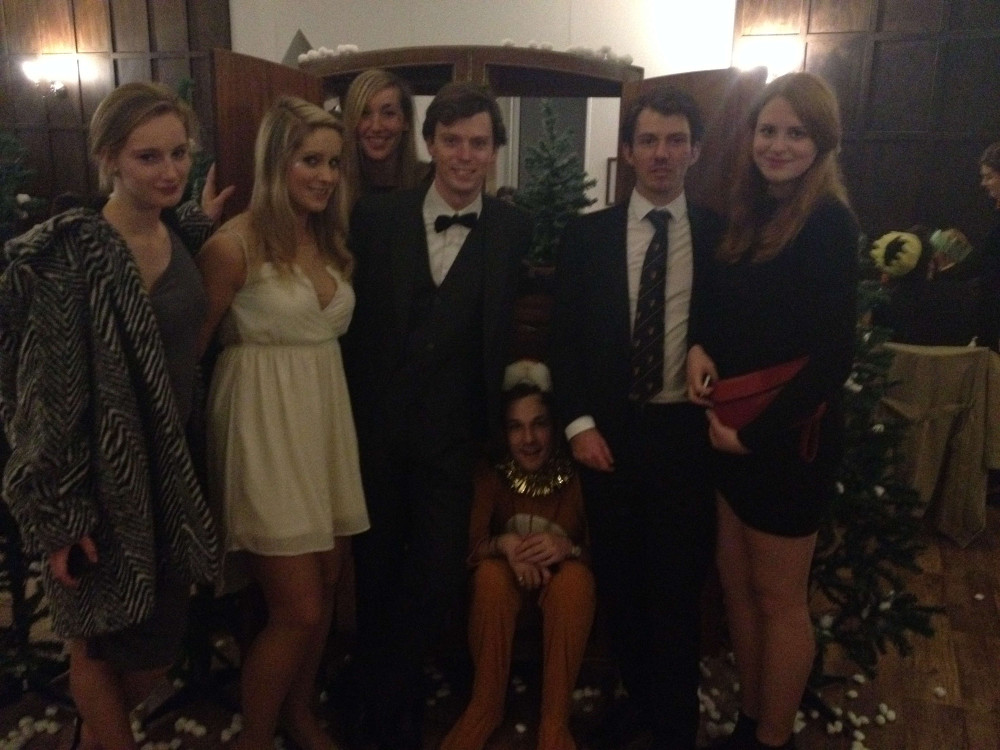
\includegraphics[width= \textwidth]{narnia.jpg}
                \caption[]{Narnia-themed End-of-term Dinner}
                \label{fig:narnia}
        \end{minipage}%
\end{figure}

\chapterimage{chapter_head_2.jpg} % Chapter heading image

\chapter{Accommodation}

The majority of New College graduate students are housed in College accommodation for their first year of graduate study with a reasonable chance of receiving second year housing. New College graduates receive some of the most desirable accommodation facilities that are provided for students living in Oxford. Graduate students are mainly housed together in the Weston buildings, with growing numbers of students living in Castle Mill and Warham House. All accommodation costs approximately \pounds140 per week.

All College-owned graduate rooms are single study bedrooms that have a wealth of facilities including desk spaces, lamps, bookshelves, internal telephone, Ethernet connection, and heaters. As of 2013, the buildings have also been fitted with wireless Internet access.  Rooms will have 240\,V electrical sockets as well as sockets for razors near the basins.

Graduate rooms are kept clean by the college scouts. The scouts tidy communal areas each weekday and thoroughly clean your room on a weekly basis. It is usual to tip your scout either at Christmas or when you leave at the end of the academic year. The scouts are an integral part of college life so please do not hesitate to introduce yourself when they come by. 

The college housing regulations state that graduates may invite guests to stay in their rooms, but only for a maximum of two nights at a time. Alternatively, students can book one of the JCR single or double guest rooms, which are available very cheaply. If you wish to book one of these rooms please contact the Home Bursar's secretary Joan Fraser (\href{mailto:joan.fraser@new.ox.ac.uk}{\urlformat{joan.fraser@new.ox.ac.uk}}), but arrange this well in advance since these rooms are very popular during each term.

\section{Weston Buildings}

The Weston Buildings are located alongside a branch of the River Cherwell at the 
College Sports Ground, which is a short seven-minute walk from the main college site. The buildings provide 96 rooms for graduate students, which are divided into 16 houses. The rooms are modern, have a sink, and are well proportioned. Each house has a large self-catered kitchen with a patio area, four toilets, and three shower rooms. Laundry facilities are located in a small building opposite House 16.

\section{Warham House}
Warham house has 9~rooms for first-year and returning graduate students. It is located on Mansfield Road about two minutes' walk from college. It has recently been refurbished to a very high standard. The rooms are mostly large, although they are all different. There are a couple of kitchens, five toilets and four bath/shower rooms. There is one washing machine and tumble dryer.

\section{Castle Mill}
Castle Mill is a university accommodation complex situated in
central west Oxford close to the Railway Station, which is a ten-minute bike ride from the college and many research buildings of
the University. Each of the newly constructed 18 bedrooms earmarked for New
College has en-suite bathroom facilities with a kitchen and dining room that is shared between
the four to six students on each floor. There are four washing machines and
dryers available on site.

\begin{figure}[htbp]
\centering
		\begin{minipage}{0.28\textwidth}
                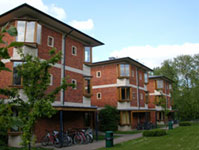
\includegraphics[width=\textwidth]{weston.jpg}
        \end{minipage}%
        \quad
        \begin{minipage}{0.28\textwidth}
                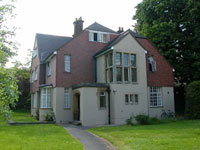
\includegraphics[width=\textwidth]{warham.jpg}
        \end{minipage}%
        \quad
        \begin{minipage}{0.35\textwidth}      
                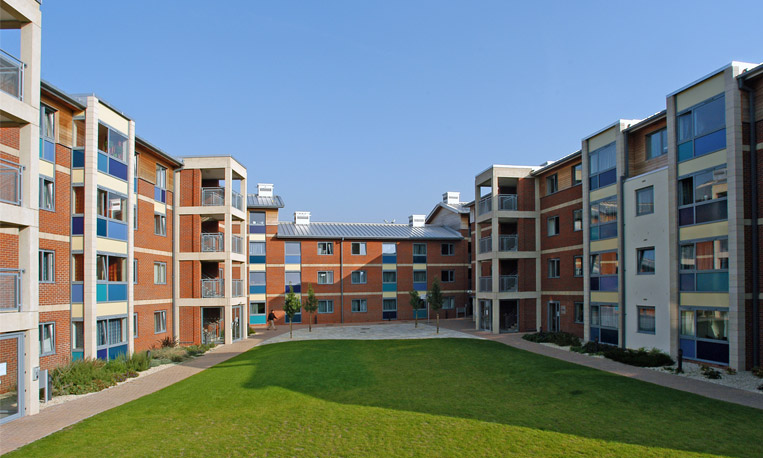
\includegraphics[width= \textwidth]{castlemill.jpg}
        \end{minipage}%
        \caption[]{The Weston complex,
        Warham house and Castle Mill accommodation sites.}
        \label{fig:accomm}
\end{figure}

\begin{figure}[htbp]
\centering
		\begin{minipage}{0.50\textwidth}
                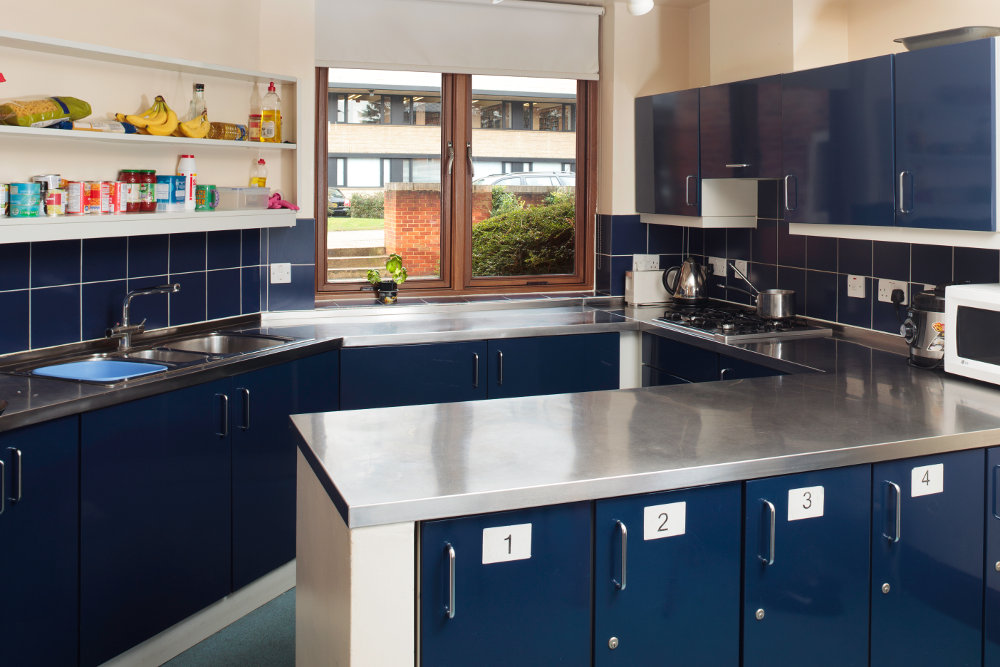
\includegraphics[width=\textwidth]{kitchen.jpg}
        \end{minipage}%
        \quad
        \begin{minipage}{0.46\textwidth}
                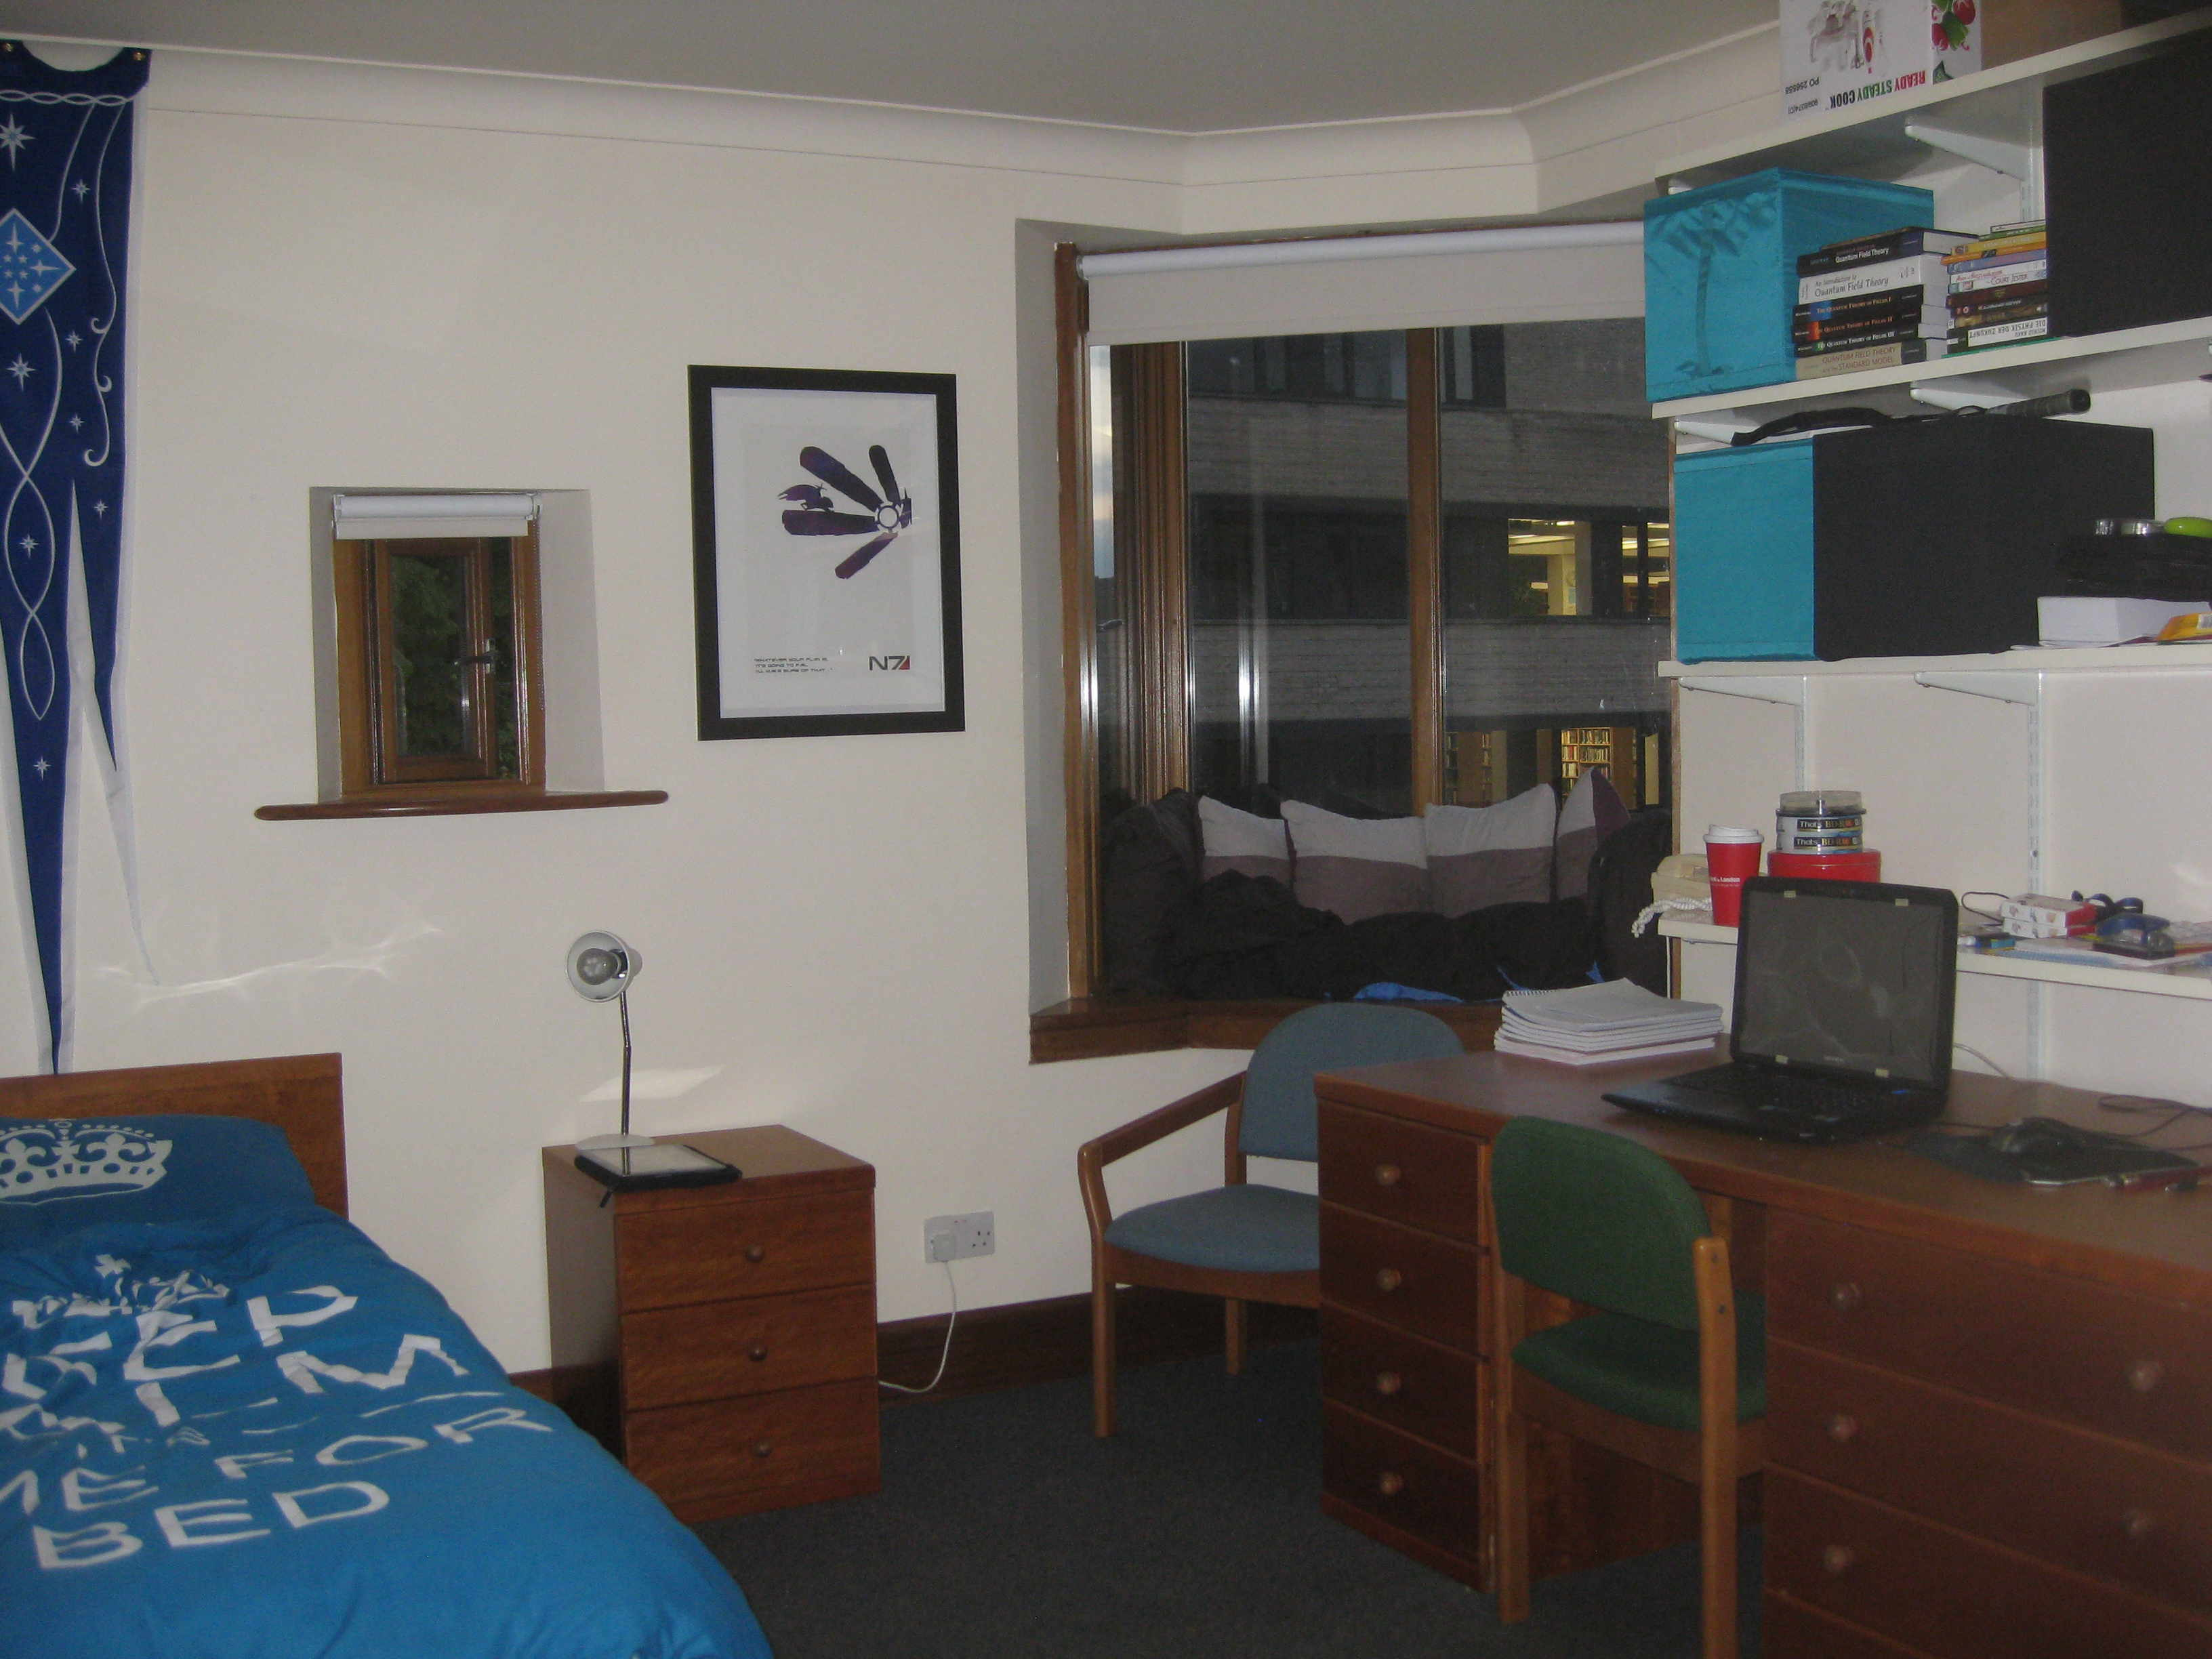
\includegraphics[width=\textwidth]{weston2.jpg}
        \end{minipage}%
\caption[]{A kitchen and a typical room
in the Weston buildings}
\label{fig:weston}
\end{figure}



\chapterimage{chapter_head_3i.jpg} % Chapter heading image

\chapter{Money}

Everything to do with money in College is in some way connected to the Bursary,
located on the ground floor of staircase~4OB. It is open weekdays between
9.30\,am and 12.30\,pm, and again between 2.15\,pm and 3.30\,pm. This is where you go to pick up grant cheques and other such payments. You can also go here to pay your battels at the beginning of each term and to add money to your till account (Bod card), but these processes are more easily done online via \url{food.new.ox.ac.uk}. You can also make payments through the golden letterbox in the wall, even when the Bursary is not open. If you have issues with payments, you can contact Linda Goodsell (\href{mailto:linda.goodsell@new.ox.ac.uk}{\urlformat{linda.goodsell@new.ox.ac.uk}}) or visit during opening hours. Bear in mind that the bursary is extremely busy in the first few weeks of term.

\section{Battels}
Have you been skipping over sentences with the word battels in them? If so, then
this paragraph is for you. Battels are your bill for accommodation, dinners and
other little things, such as some MCR events; you have to pay it at the start of each term. Accommodation is paid in advance at the beginning of the term, but dinners and other small expenses are not charged until the beginning of the next term. Your first battels will be put in your pidge, but after this it will be e-mailed to you. It is usually possible to negotiate a short extension to the payment deadline if it's really necessary. Any Junior Member who has an outstanding battels debt at Noon on the Friday of 1st Week,  and  who  has  not  seen  the  Bursar  or  emailed the  Bursary  to  agree  a timetable  for  settlement  of  this  debt,  will  be  required  to  pay  an  administrative charge of £5 and will be barred from further credit facilities within College.  Further payments will be imposed if Battels are still outstanding at Noon on Friday of 2nd Week. Battels can be paid in person at the bursary or online with your debit card (or credit card at a 1.92\% surcharge) through the \url{food.new.ox.ac.uk} website.
\section{Till account}
This is the account you use to pay for food in hall and drinks in the college
bar, which you do with your Bod-card. You \emph{CAN NOT} go in debt in the
college and MCR bars, unlike in the hall, where you can go in debt without
interests for breakfast and lunch up to \pounds15: this debt will be added to your next Battels. The easiest way top up
your account is online using the \url{food.new.ox.ac.uk} website and your debit card, however, you can also pay by cheque to the bursary.

\section[Grants and bursaries]{Travel grants, hardship grants and bursaries}
College has a research fund for graduate students. This is primarily for necessary travel (e.g. conference attendance/archival visits), but some purchases (e.g. essential software) will be considered on their merits. Taught master's students can get up to \pounds200 and research students can get \pounds375 per year (and this can accrue if not used). Medics on Electives can apply for special travel grants: \pounds750 per year for placement outside the U.K. Forms are on the college website at \url{www.new.ox.ac.uk/graduate-awards}.

There are numerous other funds for various things, particularly sport and other
\emph{meritorious} activities which will be advertised throughout the year in communication by college.. If, and only if, your circumstances change
adversely after you get to Oxford, then you are eligible for a hardship grant from The College Financial Aid Committee. Make an appointment with the bursar, who is usually very helpful if you are in genuine need.

Outside of College, those experiencing unexpected financial difficulties can also apply to the University Hardship Fund (\url{http://www.ox.ac.uk/students/fees-funding/assistance/hardship/uhf}) by the fourth week of each term. UK students can also apply to the Access to Learning Fund (\url{thttp://www.ox.ac.uk/students/fees-funding/assistance/hardship/alf}). The University website has further information on possible sources of financial support at \url{www.ox.ac.uk/feesandfunding/graduates} and OUSU offers an advice service (\url{advice@ousu.org}).

There are some other bursaries and small pots of money which may be available. a list of these is on the college website at \url{www.new.ox.ac.uk/graduate-awards}. You can apply for them via the Bursar, David Palfreyman (\href{mailto:bursar@new.ox.ac.uk}{\urlformat{bursar@new.ox.ac.uk}})

\section{Earning money}
You are primarily in Oxford to study and your supervisors will expect you to spend most of your time learning or doing research. However, there are opportunities to do part-time work. There are part-time opportunities in town, shifts in the college library, etc.

There are also teaching opportunities, although you are not required to teach,
and no one is guaranteed to get a teaching opportunity. Graduate students can
take undergraduate tutorials and some may even be appointed to \emph{college
lectureships}. Scientists also have the opportunity to demonstrate in practical sessions. Talk to your supervisor if you are interested in teaching.


\chapterimage{chapter_head_4.jpg} % Chapter heading image

\chapter{Essential admin after arrival}

\section{Room key}
The first thing to do when you arrive is to go to the main porters' lodge, next
to the Holywell Street entrance to New College, where the porters will tell you where you will be living and where you collect your room key. 
\section{Bod-card}
Your Bodleian reader card, always referred to as your \emph{Bod-card}, is effectively
your university card. You need it to get into college and college buildings, buy food in hall, drinks in the bar and to get into most buildings and departments across the university. It is therefore something you need to get hold of as soon as possible. You can collect your Bod card from the graduate office in 4OB3 as soon as you arrive.
\section{E-mail lists}
E-mail is the standard form of communication within the university, and you should check your account regularly. You must activate your college email address as soon as possible after arrival. There are two e-mail lists in college which you need to know about:
\begin{enumerate}
  \item Main list: The main list is run by college and important
information is sent out using it. E-mails come through with the subject line
\emph{[new-mcr]}. College should sign you up to it but inevitably they miss a
few people. If you don't seem to receive any e-mails with this subject, report it to the College IT support (\href{mailto:it-support@new.ox.ac.uk}{\urlformat{it-support@new.ox.ac.uk}}), because you need to be on this list.
  \item Social list: This list is administered by the MCR Secretary and has subject line
\emph{[newmcr-l]}. It is used by the president, vice-president, social secretaries, welfare rep and sports rep for
sending out notices and information about what is happening in the MCR. We will
try and add you automatically, but a lot of people don't get signed up, so you
should do this yourself. E-mail
\href{mailto:newmcr-l-subscribe@maillist.ox.ac.uk }{\urlformat{newmcr-l-subscribe@maillist.ox.ac.uk}}
from any e-mail account to be added to the list. In order to unsubscribe you can
e-mail
\href{mailto:newmcr-l-unsubscribe@maillist.ox.ac.uk}{\urlformat{newmcr-l-unsubscribe@maillist.ox.ac.uk}}.
\end{enumerate}


\chapterimage{chapter_head_1.jpg} % Chapter heading image

\chapter{Local information}

\section{Things to bring}

\begin{description}
  \item[For your room:] For your room: Extension cords and multi-plugs are a good idea, given the rather quaint notions the college holds about electricity. Transformers which convert cycles as well as volts will also be needed for any electrical goods purchased overseas. It also might be worthwhile to bring transformers and conversion plugs. College no longer provides pillows, sheets and duvets for the beds, so remember these or you'll be turning your clothes into a make-shift pillow on the first night.
  
  \item[For the kitchen:] You will need to bring or buy your own plates, bowls, mugs, glasses, cutlery and storage containers. Sandwich toasters, bottle openers and the like can be especially handy. College DOES provide kitchens with a microwave, a toaster and a kettle. Boswells and other general goods stores in Oxford offer discounts on all home-ware purchases in the first few weeks of term on presentation of your Bod card. Robert Dyas is a good bet as they do a year-round student discount. Your kitchen may have some of these items left over from previous students, and your kitchen-mates may be happy to share what they have: check before you spend!
  
  \item[Clothes:] Despite the impression given by the photos in this guide, it is not always sunny. So, apart from the required academic dress (see below), perhaps the most important items to remember are warm clothes for the winter. There will be a few formal occasions when College serves up its finest cuisine, and many more optional black tie events besides, so pack some classy clothes. For
men, there are many opportunities to wear dinner suits and although it is easily possible to get by without one, if you bring one or buy one in Oxford you will get good use out of it.

  \end{description}
\section{Gowns and academic dress}\label{AcaDress}
One of the classic images of Oxford is students going around in gowns and academic dress. You also need a gown for dining at formal hall and various other occasions in college; at New College it can just be worn over normal clothes for formal hall. Most graduate students will wear a graduate gown, although you can wear the gown of your old university. 

You need academic dress, called sub fusc, for formal university events such as
matriculation, university exams and research degree vivas as well as for
graduation. This is special clothing that is worn underneath your gown. 
\begin{itemize}

\item \emph{one of}: 
\begin{itemize}
\item dark suit with dark socks, or
\item dark skirt with black tights and stockings, or
\item dark trousers with dark socks or dark hosiery
\end{itemize}
\item dark coat if required
\item black shoes
\item plan white collared shirt or blouse
\item white bow tie, black bow tie, black full-length tie, or black ribbon
\end{itemize}

You also need a mortarboard, but you might want to choose the less common soft cap as an alternative, which was traditionally worn by women. There are outfitters around town (Shepherd \& Woodward, Walter's) who provide a gown, mortarboard and white bow tie/black ribbon, usually as some part of package deal in the first couple of weeks of term.


\begin{figure}[htbp]
\centering
		\begin{minipage}{0.58\textwidth}
        	\centering
				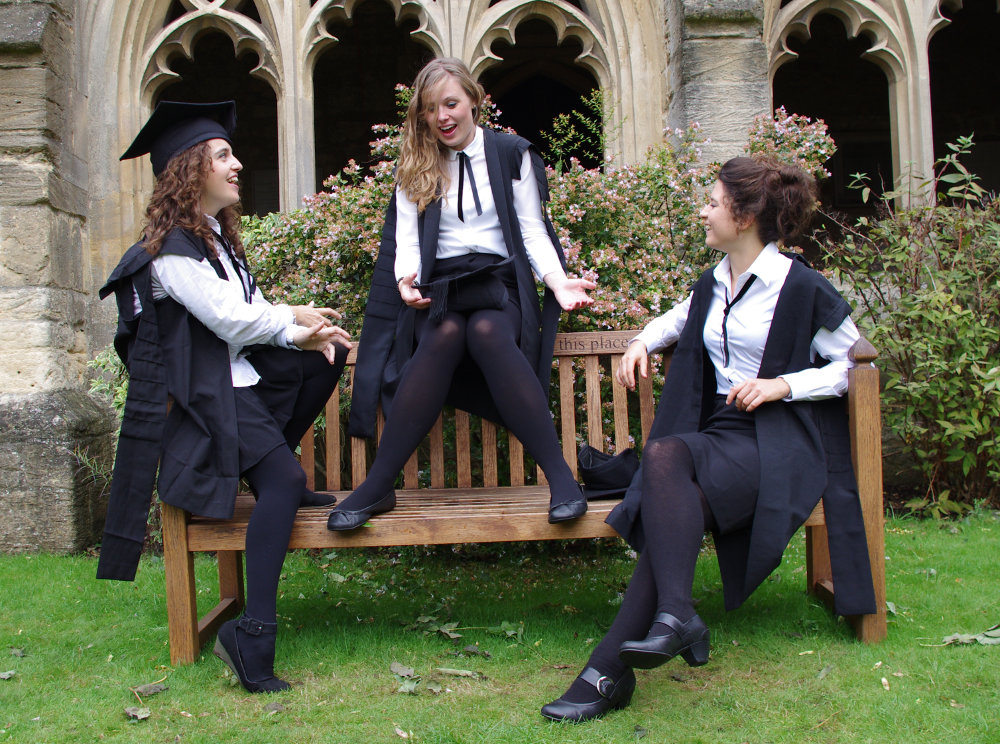
\includegraphics[width=0.9\textwidth]{subfusc2.jpg}
				\caption[]{Oxford natives in traditional costumes}
				\label{fig:subfusc}
        \end{minipage}%
        \quad
		\begin{minipage}{0.38\textwidth}
        	\centering
				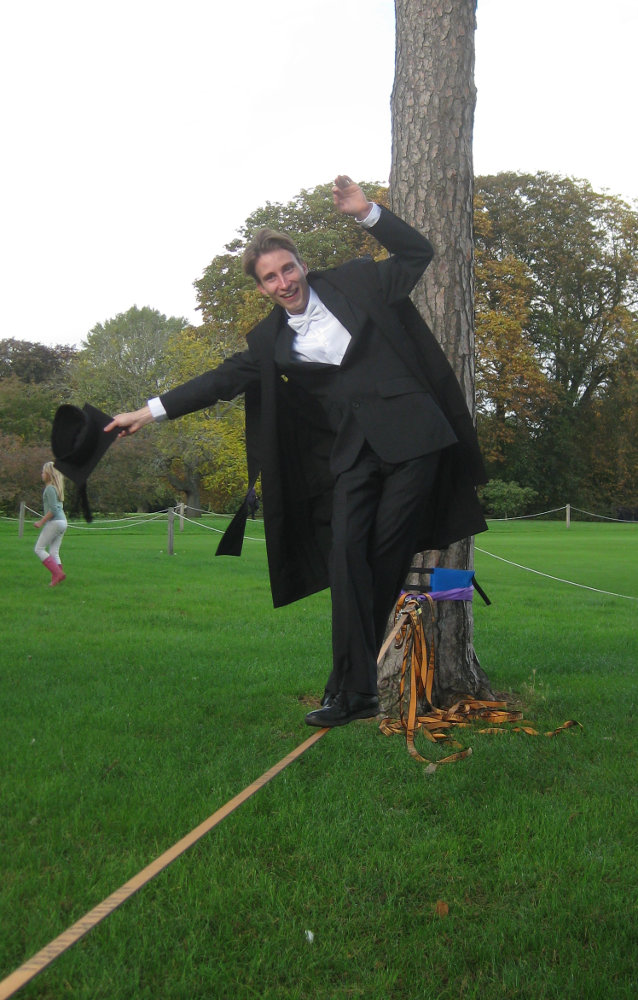
\includegraphics[width=0.9\textwidth]{subfusc.jpg}
				\caption[]{\emph{EVERYTHING} in Oxford is done in sub fusc and
				gown!}
				\label{fig:slack}
        \end{minipage}%
\end{figure}  
  
\section{Bicycles}
Some people cannot live without their bike in Oxford, whilst others get by fine
without one. A lot depends on your lifestyle, particularly the distance between
your accommodation and where you will be spending most of your time working
(department/lab/favourite library). Buying a new bike in Oxford can be expensive
but due to the high bike-to-person ratio there is a large second-hand market.
The \href{http://www.dailyinfo.co.uk/}{\urlformat{DailyInfo}} website is a good place to start looking (as are the usual websites such as Gumtree), and expect to pay more than \pounds50. Bike theft is
the most common crime committed against Oxford students, so a high-quality
D-lock is essential (\pounds15 for students
\url{https://www.admin.ox.ac.uk/ouss/cra/cyclesecurity/}).

\section{Welfare}
College provides a constellation of people attuned to all manner of welfare matters: there are the Cox and Salvesen Fellows, both experts in the ways of pastoral care; the Chaplain, who can advise on any issue, spiritual or otherwise; the porters, frequently indispensable in times of need; the Dean, the Assistant Dean, and the two Junior Deans; as well as our MCR welfare officer and trained peer supporters. See below for contact information.

\medskip

\begin{table}[!h]
\centering
\begin{tabular}{ >{\bfseries}l l}
\toprule
Welfare Contacts & Telephone and e-mail \\
\midrule
Main Porters' Lodge	&			(01865~2)79500 \\
Weston Porters' Lodge	&		(01865~2)81081 \\
Nightline (8\,pm-8\,am, 0th-9th week) &	(01865~2)70270 \\
Counselling Service & 			(01865~2)70300\\
					&			\href{mailto:reception@counserv.ox.ac.uk}{\urlformat{reception@counserv.ox.ac.uk}} \\
Student Advice Service &		\href{mailto:advice@ousu.org}{\urlformat{advice@ousu.org}} \\
Emergency				&		999\\
\bottomrule
\end{tabular}
\caption{Welfare Contacts}
\label{tab:welfcontact}
\end{table}

\begin{table}[!h]
\centering
\begin{tabular}{ >{\bfseries}l l}
\toprule
New College Welfare Team & Telephone and e-mail \\
\midrule
Erica Longfellow, Chaplain (3OB6)	& (01865~2)79451 \\
						& \href{mailto:erica.longfellow@new.ox.ac.uk}{\urlformat{erica.longfellow@new.ox.ac.uk}} \\
Tom Cutterham, Cox Fellow &			(01865~2)79514 \\
						& \href{mailto:tom.cutterham@new.ox.ac.uk}{\urlformat{tom.cutterham@new.ox.ac.uk}} \\
Ryan Hanley, Salvesen Fellow & 		(01865~2)79531 \\
						& \href{mailto:ryan.hanley@new.ox.ac.uk}{\urlformat{ryan.hanley@new.ox.ac.uk}} \\
Caroline Thomas, Domestic Bursar &	(01865~2)79560 \\
						& \href{mailto:caroline.thomas@new.ox.ac.uk}{\urlformat{caroline.thomas@new.ox.ac.uk}}\\ 
\bottomrule
\end{tabular}
\caption{New College Welfare Team}
\label{tab:welfcollege}
\end{table}

\begin{table}[!h]
\centering
\begin{tabular}{ >{\bfseries}l l}
\toprule
MCR Peer Supporters & e-mail \\
\midrule

Belinda Faust (Welfare Officer)	& \href{mailto:belinda.faust@new.ox.ac.uk}{\urlformat{belinda.faust@new.ox.ac.uk}} \\
Martin Hallmannsecker (LGBTQ+ officer) & \href{mailto:martin.hallmannsecker@new.ox.ac.uk}{\urlformat{martin.hallmannsecker@new.ox.ac.uk}} \\
Cristina Golomoz (Women's Officer)	& \href{mailto:cristina.golomoz@new.ox.ac.uk}{\urlformat{cristina.golomoz@new.ox.ac.uk}} \\
Erika Lam (Peer Supporter)	& \href{mailto:erika.lam@new.ox.ac.uk}{\urlformat{erika.lam@new.ox.ac.uk}} \\
Richard Millar (Peer Supporter)	& \href{mailto:richard.millar@new.ox.ac.uk}{\urlformat{richard.millar@new.ox.ac.uk}} \\
\bottomrule
\end{tabular}
\caption{Peer Supporters}
\label{tab:peersupp}
\end{table}

Please note that the phone numbers without brackets are from internal lines (e.g. using the phone in your room at Weston). From outside lines, including your own mobile, dial the area code 01865, then 2 and then the number. Please make an appointment in advance (preferably via email) to see the Cox or the Salvesen Fellow. In an emergency, however, contact the Porters' Lodge and they will get in touch with a member of the welfare team for you straight away

\section{LGBTQ+ students}
There is a lot going on at Oxford for lesbian, gay, bisexual, transexual and
intersex students. The College may date from 1379, and the University from about
200 years before that, but you'll find that attitudes have moved on a long way
since then. There are LGBTQ students in the New College MCR and all across the
town and University, so there will be plenty of friendly faces to show you the
sights and give you the insiders' tips on the best places to go out.
Alternatively, get in touch with the lovely Hamish
(\href{mailto:martin.hallmannsecker@new.ox.ac.uk}{\urlformat{martin.hallmannsecker@new.ox.ac.uk}}), your very own LGBTQ+ rep on the MCR committee, who keeps you updated with all the weekly events and is always approachable in case you need someone to talk to. OU LGBTQ+ Society (\url{http:// oulgbtsoc.com}) has heaps of info on their website, and is a great group to join with lots of fun social events. Keep your eyes out for the OUSU LGBT handbook, and OUSU also have a Queer Rights group if you are interested in the more activist side of things. More information on freshers' events outside college will be available in freshers' fortnight.

\section{Terms}
Oxford has three terms: Michaelmas from October to December; Hilary from January
to March; Trinity from April to June. Terms formally last eight weeks: weeks
'start' on Sunday and are numbered from one through to eight. Thus, within
Oxford, you tend to describe dates using this system: so, for example, you might
say, \emph{my exam is on Tuesday of 7th week}. The week before first is called
0th week and the one before that minus 1st week etc. The gaps between terms are the \emph{Christmas}, \emph{Easter} and \emph{Long} vacations.
\medskip

Undergraduate teaching takes place during weeks of full term. For those doing taught courses, teaching will be focused during term but you may well have to do assignments out of term: so check this before you book a six week holiday in the Easter vacation! For research students terms are less relevant, and what time you get away is largely up to you and your supervisor.

\section{Transportation}

The public transport system in and around Oxford relies mainly on the
\href{http://www.oxfordbus.co.uk/}{\urlformat{Oxford Bus Company}} buses, the
single fare in the centre region is \pounds1, to be paid to the driver (they
prefer exact change).

The main connections to London are run by the
\href{http://www.oxfordtube.com/}{\urlformat{Oxford Tube}}, a bus line from
Oxford's central bus station at Gloucester Green to London Victoria, and
\href{https://www.firstgreatwestern.co.uk/}{\urlformat{First Great Western}},
the train carrier connecting Oxford to London Paddington. Both offer various fares depending on booking date,
return date, number of tickets bought, etc. The cheapest fare for both of them
is \pounds10-12 for a return ticket, but the availability conditions
vary.

There is now also a new train connection between Oxford and London Marleybone run by \href{https://www.chilternrailways.co.uk/}{\urlformat{Chiltern Railways}}. 

Luton and Standsted airports can be reached by bus via
\href{http://www.nationalexpress.com/}{\urlformat{National Express}}, Heathrow
and Gatwick via the \href{http://airline.oxfordbus.co.uk/}{\urlformat{Airline}},
a bus operated by the Oxford Bus Company.
Tickets for all of them can be bought via the
\href{http://www.nationalexpress.com/}{\urlformat{National Express page}}, the
Airline tickets also via the \href{https://airlinebooking.oxfordbus.co.uk/}{\urlformat{Airline page}}.
Fares vary depending on time of day, advance booking, return dates and other
more mysterious criteria. A single trip to Luton costs up to \pounds18, to
Heathrow up to \pounds25, to Stansted up to \pounds27 and to Gatwick up to \pounds30,
return and off peak tickets are often cheaper.
In many cases creative routes can lower the costs (e.g. taking the bus from
Gatwick to Victoria, followed by the Oxford Tube to Oxford comes to \pounds21),
as can
\href{http://www.nationalexpress.com/waystosave/young-persons-coachcard.aspx}
{\urlformat{Coachcards}}
and \href{http://www.railcard.co.uk/}{\urlformat{Railcards}}, which allow you to
save a fixed percentage of the fare for many routes. Their usefulness depends heavily on your travel style, but they may be worth a look.


\chapterimage{chapter_head_2.jpg} % Chapter heading image

\chapter{Information for Overseas Students}
\enlargethispage{\baselineskip}

See also: \url{http://www.ox.ac.uk/students/new/international}

\section{Banking} 

The following banks have branches in central Oxford:
\begin{itemize}
  \item Barclays: 54 Cornmarket Street
  \item The Cooperative Bank: 13 New Road
  \item Halifax: 13A New Road
  \item HSBC: 65 Cornmarket Street  
  \item Lloyds: corner of High, Cornmarket, Queen, and St Aldate's Streets. 
  \item NatWest: 121 High Street and corner of Cornmarket and George Street
  \item Royal Bank of Scotland: corner of St Giles and Little Clarendon Street.
  \item Nationwide:44 Queen Street
  \item Santander: 114 St Aldate's Street
  \item TSB Bank: 17 George Street
\end{itemize}

The details of bank accounts change rapidly; an up-to-date comparison of student accounts can be found at: 
\url{http://www.savethestudent.org/money/student-banking/student-bank-accounts.html} 

Opening an account is surprisingly difficult. It is worth asking your bank at home if they can set up an account for you with an English bank (or another agency such as Thomas Cook in Australia). When opening your bank account, you will usually need:
\begin{itemize}
  \item A means of proving your identity and immigration status: your
passport with visa OR your EU national photo ID (whichever is applicable),
 \item Proof of your UK address: your admissions letter from College should do
 this as well (at least in the first weeks of term). Sometimes banks will be difficult about this, demanding bills which you logically will not yet have; this may be a sign that they are not the bank for you. 
 \item It may also be necessary to provide details of your previous bank
 accounts (i.e. a statement) 
\end{itemize}

Many of the banks will have stalls at the International Students' Orientation with exact descriptions of their current requirements.

Once you have opened an account, it can take weeks before your cheque book, debit card, cheque guarantee card (essential for payment by cheque), or credit card are available. Likewise, expect all deposits (except cash) to take up to one week before funds are made available to you. 

Bureau de Change counters are available in every bank for converting currencies.There are both American Express and Thomas Cook offices on Queen Street. Marks and Spencer on Queen Street also offers a currency exchange, as does the exchange service at the tourist information on Broad Street.

Many overseas students have found it difficult, costly, and time-consuming to
access funds from their home countries. Ideally, arrange to arrive in the UK
with a certified cheque issued by your bank already in Pounds Sterling for
however much of your money you wish to have available here. Most ATMs accept
overseas debit cards, allowing you to withdraw cash from your account back home,
but your bank will usually charge you for this. Credit cards are similarly
useful, although the fees and interest costs are potentially prohibitive. There
is also a policy of not issuing international students with a UK credit card
until they have been in the UK for at least 6 months. You can arrange with the
New College Bursary to pay your fees by international wire transfer. Information
on this process will be sent to you with your bill each time it is due. 

\section{Electricity and appliances} With the proper precautions and planning,
you should be able to bring most of your electrical appliances with you to Oxford. Be forewarned, however, that the UK's different electrical current and cycle rate has cost many the ill-prepared graduate some piece of much-loved equipment.

Electricity in the UK operates on a AC~220-240\,V, 50\,Hz system. If your
equipment is designed to run in a range that includes both these figures, you
simply need to purchase an adaptor which will allow you to fit your devices'
plug(s) to the wall outlets here. Check your devices' specifications. Many
recent computers, for instance, are designed to be used in 110-240\,V, 50-60\,Hz
ranges, thus requiring nothing more than an adaptor for use here.
These can be picked up at any number of stores in Oxford during your first weeks
here (Boswells on Broad Street is a good all-purpose department store).

If your equipment is not rated for the UK electrical system, you will need to
purchase a transformer which will alter the electrical current used in the UK to
the appropriate current for your equipment. American products, for example, are
usually built for AC~110\,V, 60\,Hz. While almost all transformers will easily
handle the step down from 220\,V to 110\,V, only very expensive ones will change
the cycle rate, ie the 50\,Hz to 60\,Hz. Any equipment that needs to run
constantly at a certain speed from an internal motor (e.g. CD players, blenders, cassette tape players, and clocks) may not work here, and may be damaged through trying them. Again, if in doubt, check your products' specifications and inquire at the dealer or manufacturer.

If your equipment will work with a transformer, make sure you get one that is powerful enough for everything that you plan to use. Transformers can only handle a certain amount of wattage. Add up the total amount of watts used by all of your equipment and make sure it is less than your transformer can handle, or you'll fry your transformer and potentially destroy your equipment. The Oxford University Computing Centre at 13 Banbury Road sells transformers although you would be best advised to pick them up in your home country before you arrive.

If you are living in College, there are a wide range of restrictions on your use
of electrical appliances: see the
\href{http://www.new.ox.ac.uk/sites/default/files/sites/all/files/HB_Web version_100915.pdf}{\urlformat{Dean's Handbook}}, 4f (pg. 27).

\section{Work} 
The \href{http://www.ox.ac.uk/about/international-oxford}{\urlformat{International Student Office}} which runs an Orientation programme for all international students at the start of your Oxford career, will be your best and primary resource for advice on visas, work permits, funding, etc.
Citizens of the UK, EEA and Switzerland have no work restrictions. Holders of
Tier 4 visas are restricted - your passport sticker should state the exact
restrictions (see here:
\url{http://www.ukcisa.org.uk/Information--Advice/Working/Can-you-work layer-5316}). These restrictions apply to paid teaching or pastoral work undertaken for a College or the University.
The UK government has a scheme for doctoral students to stay in the UK to work
after finishing a degree, and full details can be found on their website:
\url{http://www.ukcisa.org.uk/Information--Advice/Working/Working-after-studies layer-3780/}.
The \href{http://www.careers.ox.ac.uk/}{\urlformat{University Careers Service}} offers sessions and resources on working internationally or staying to work in the UK.

\section{Health care}
See also 
\begin{itemize}
  \item \url{http://www.new.ox.ac.uk/international-visiting-students}
  \item \url{http://www.nhs.uk/NHSENGLAND/Pages/NHSEngland.aspx}
\end{itemize}

New College has its own GP (medical doctor) on 28~Beaumont Street; you will be signed up for this service during College orientation.  
NHS provides free emergency care for all. However, unless you are a citizen of
the UK, the EEA, Switzerland, Australia, New Zealand or the Falkland Islands,
you will have to pay a \emph{Health surcharge} of \pounds150 per year, as part of
your visa in order to get access to non-emergency NHS services. You cannot opt out of this.
With that paid, you will have a right to free hospital care, free visits to your
GP, subsidised prescriptions (\pounds8.20 for most medicine), and subsidised
dental care. Sight tests, contact lenses and glasses are not covered by NHS.


\section{Mobile phones} 

The UK is a very mobile-phone-centred nation and you will really need a mobile to stay in touch with friends while here. Most Brits use texts (also known as SMS) or phone-based internet chat as their main form of communication, since these are cheaper than calls. 
If you don't bring a telephone to Oxford from your home country which will work in the UK, you can purchase a phone at any of the telephone retailers - most of which are located on Cornmarket Street (Vodafone, Orange, O2, etc). These retailers can also provide you with telephone service for your mobile. There are two main types of payment for mobile phone usage:

\begin{enumerate}
  \item \textbf{Pay as you go plan.} This means that you deposit money
towards your phone account and can make calls and texts until your money runs out.
 \item \textbf{Pay monthly.}  You pay a certain amount a month, for which you
get set amounts (sometimes unlimited) of minutes for calls, texts, and internet
allowance. The amount of each you get depends on how much you are willing to pay
per month! Without a bank account and/or proof of steady income, you will most
likely not qualify for the \emph{pay monthly} option, and will have to purchase a
\emph{pay as you go} plan. It is highly recommended therefore that, after you
have your bank account set up, you go and sign up for a monthly contract rather than a pay as you go plan.
\end{enumerate}


 

%\setcounter{nosmtoc}{1} %switches small table of contents off
%\chapterimage{chapter_head_3i.jpg} % Chapter heading image

\chapter{Glossary of Oxford Terminology}

As you will have gathered if you have read this far, Oxford has much terminology which is not often heard outside its grey walls. The following is a list of a few of them.

\begin{description}
\item[Balls] Virtually every college has a ball (some smaller ones are called events). They vary greatly in scale. New College rotates hosting the commemoration ball every three years with Magdalen and Worcester. New College is hosting the commemoration ball in 2016!
\item[Battels] The bill you receive from College for the various debts you will
have incurred, i.e. drinks, chocolate, Guest Night dinners, accommodation.
\item[Black Tie Dress] \emph{Men}: dinner suit (tuxedo), though you can usually
get away with wearing a black suit, with a bow tie of any colour apart from
white; \emph{women}: stylish cocktail-length or long dress or equivalent.
\item[Blue] University award for being a jolly good sport in something like
rowing or cricket.
\item[Boat Race] The famous competition between Oxford and The Other Place (see
\emph{Cambridge}) rowing eights in London.
\item[The Bod] The Bodleian Library. Not merely the glorious building housing
the oldest library in the English-speaking world, but now something resembling a huge multinational corporation that controls all the books in Oxford.
\item[Bop] A college party.
\item[Bumps] A type of rowing race.
\item[Cambridge] A town somewhere to the north-east of Oxford where there is
another university. Commonly referred to as \emph{The Other Place}, and those
who study there are known as \emph{Tabs} (short for \emph{Cantabs}).
\item[Cherwell] A pleasant tributary of the Isis (Thames), upon which you will
spend most of your summer punting.
\item[Coming up] Opposite of going down.
\item[Cuppers] A competition between different colleges at sport.
\item[Dean's handbook] Your bible for all college related rules, to be found at
\url{http://www.new.ox.ac.uk/deans-handbook}
\item[Don] An academic.
\item[Eight] A type of boat you row.
\item[Eights week] The week in Trinity during which \emph{Summer eights} are
held.
\item[Fellow] Most academics are fellows of a college and are involved in its
governance.
\item[Fresher] A new student, whether undergraduate or grad.
\item[Front Quad] New College's oldest quad. The lodge is no longer
here, though, so it is no longer at the front\ldots
\item[Going down] Depends on the context, but it can mean to leave Oxford.
\item[High table] Where the fellows of the college eat dinner. Students may
occasionally be invited to join them. Students generally eat at common table.
\item[Hilary term] Term running from January to March. 
\item[Isis] The big river in Oxford. This is the same river that elsewhere is
called the Thames.
However, where it flows through Oxford it is called the Isis - it is incorrect to use Thames.
\item[JCR] Junior Common Room. The undergraduate body of students and their
physical common room. Graduate students are members of this.
\item[JRF] Junior Research Fellow. Similar to a post-doc. Usually funded from
the college's endowment.
\item[Long vacation] Summer vacation between June and October. 
\item[Matriculation] Ceremony where you formally become part of the university
and promise not to burn the books in the Bodleian. Done in sub fusc at the end of 1st week in Michealmas.
\item[MCR] Middle Common Room.
\item[Michaelmas] The term between October and December.
\item[New Buildings] New Buildings~(NB) are in the Holywell Quad. The porters'
lodge is there and some lecture rooms but it is mainly undergraduate accommodation.
\item[New College] The best college in Oxford. 
\item[Old buildings] Old buildings~(OB) is the name given to the staircases in
both the Front Quad and the Garden Quad.
\item[OUSU] The Oxford University Students Union.
\item[Oxford Blue] A colour.
\item[Oxford Union] Often shortened to \emph{The Union}. A world famous debating
society, connected to the university. Beer is \pounds1 a pint, and membership
fee is above \pounds200 - at least the priorities are clear.
\item[The University Parks] A large park owned by the University containing one
of the best cricket grounds in the country.
\item[Pigeon post] The internal mail. 
\item[Porters' lodge] Where you find porters, and your post (in the post room). 
\item[Proctors] Academics who are responsible for discipline and welfare across
the University.
\item[Punting] A way to move around on water and something to spend summer
doing.
\item[Quad] Short for quadrangle. A roughly square-shaped space, surrounded by
buildings. Called \emph{court} in The Other Place.
\item[Rad Cam] The Radcliffe Camera, part of the Bodleian library. 
\item[Rustication] Not quite expelled, but sent to live far away from College
while still studying at Oxford as a result of having done a bad, bad thing. 
\item[Scout] The person who cleans your room. Be very nice to them.
\item[SCR] The senior common room. Where fellows, and other senior college
officers, eat and socalise. Also a collective name for the fellows.
\item[Sent down] To be expelled. 
\item[Sub fusc] Academic dress. 
\item[Torpids] A rowing competition between colleges in Hilary. 
\item[Town] Anything or anyone not part of the University. 
\item[Trinity] The term between April and June. Also a college. 
\item[Varsity] Used to describe a sporting contest between Oxford and The Other
Place.
\item[White tie] A dress code for events which are more formal than black tie. A
couple of balls each year are white tie, including the New College ball. For men it means a dress coat and white bow tie. For women it generally means full-length ball gowns.
\item[Wykkie Bear] The MCR mascot. Add him on Facebook!
\end{description}

\begin{figure}[htbp]
\centering
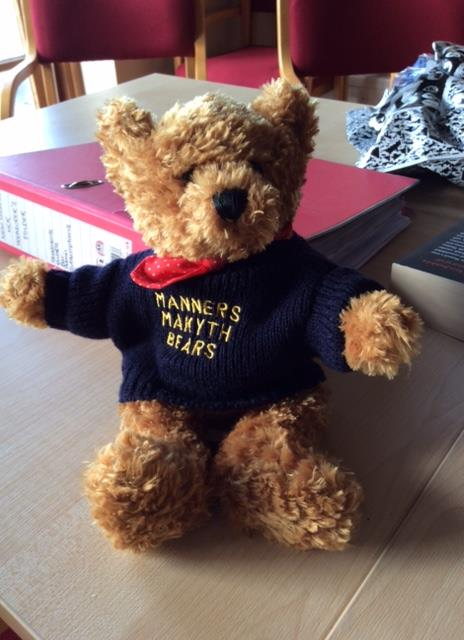
\includegraphics[width=.6\textwidth]{bear.jpg}
\caption[]{\emph{Ursus
wykehamensis collegiumnovi}, rare type of ursid, lives in the beams of
the \emph{Spoom}}
\label{fig:bear}
\end{figure}
%\setcounter{nosmtoc}{0}  %switches small table of contents on 

%\cleardoublepage
%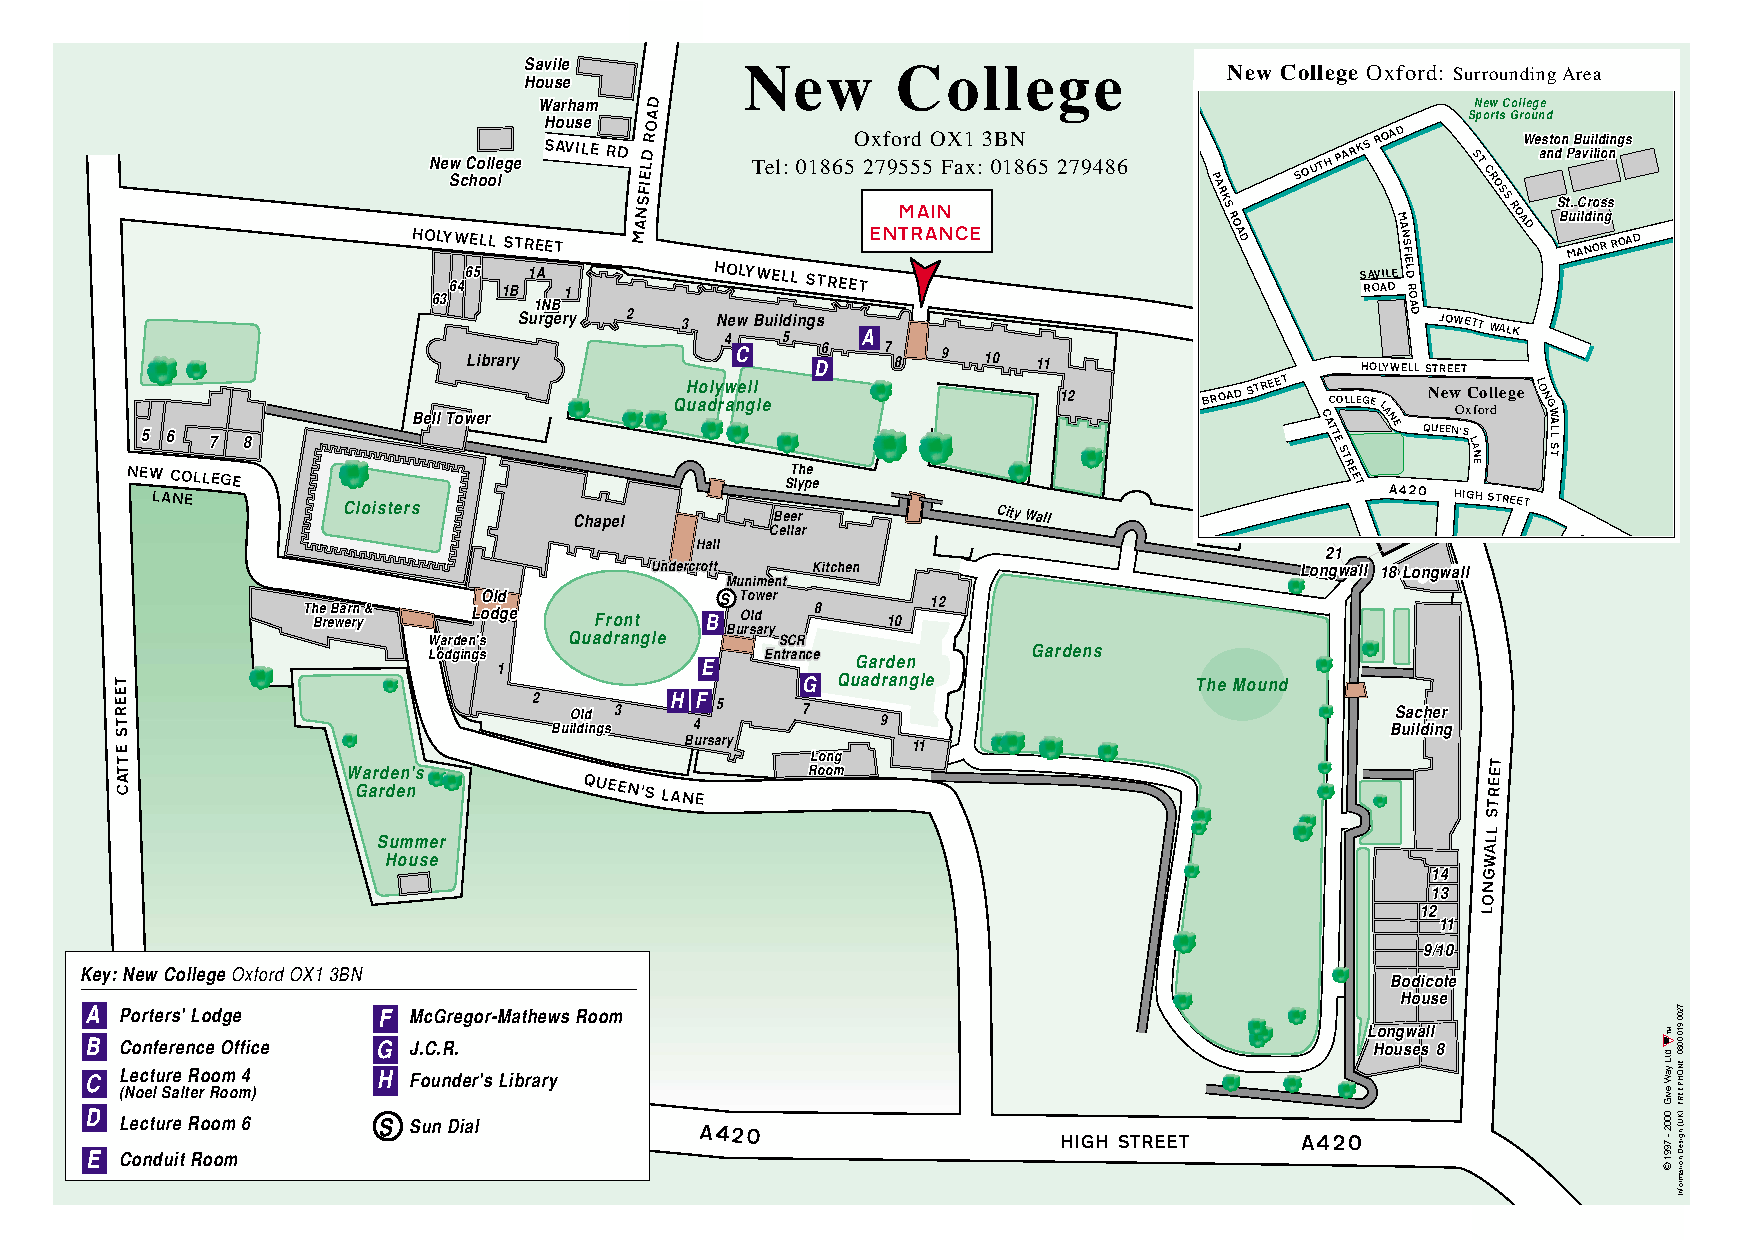
\includepdf[addtotoc={1, chapter, 1, Map of New
%College, Map},landscape=true]{./Pictures/CollegeMap.pdf}

\restoregeometry
%----------------------------------------------------------------------------------------

\end{document}